%% General document settings — ICS-lab template style
\documentclass[a4paper,10pt]{report}
\PassOptionsToPackage{nopatch=footnote}{microtype}
\usepackage{esibot}

% ── Acronyms ─────────────────────────────────────────────────────────────────
\newacronym{ros}{ROS}{Robot Operating System}
\newacronym{slam}{SLAM}{Simultaneous Localization and Mapping}
\newacronym{mcu}{MCU}{Microcontroller Unit}
\newacronym{pwm}{PWM}{Pulse-Width Modulation}
\newacronym{uart}{UART}{Universal Asynchronous Receiver-Transmitter}
\newacronym{wifi}{WiFi}{Wireless Fidelity (IEEE 802.11)}
\newacronym{urdf}{URDF}{Unified Robot Description Format}
\newacronym{tf}{TF}{Transform Tree}
\newacronym{imu}{IMU}{Inertial Measurement Unit}
\newacronym{pid}{PID}{Proportional-Integral-Derivative}
\newacronym{mjpeg}{MJPEG}{Motion JPEG}
\newacronym{gpio}{GPIO}{General-Purpose Input/Output}
\newacronym{iot}{IoT}{Internet of Things}
\newacronym{cad}{CAD}{Computer-Aided Design}
\newacronym{pla}{PLA}{Polylactic Acid}
\newacronym{amcl}{AMCL}{Adaptive Monte Carlo Localization}
\newacronym{dwb}{DWB}{Dynamic Window-Based local planner}
\newacronym{rviz}{RViz2}{ROS Visualisation tool (v2)}
\newacronym{ekf}{EKF}{Extended Kalman Filter}
\newacronym{rgbd}{RGB-D}{Red-Green-Blue + Depth (camera)}
\newacronym{i2c}{I2C}{Inter-Integrated Circuit bus}
\newacronym{cpr}{CPR}{Counts Per Revolution}
\newacronym{rpi}{RPi}{Raspberry Pi}
\newacronym{sbc}{SBC}{Single-Board Computer}
\newacronym{occgrid}{OccupancyGrid}{probabilistic 2D occupancy grid}
\newacronym{bt}{BT}{Behavior Tree}
\newacronym{cli}{CLI}{Command-Line Interface}

\title{}
\date{}
\author{}

\begin{document}

\newgeometry{top=0.6in,bottom=2.5cm,right=2.5cm,left=2.5cm,footskip=0.8cm}

\begin{titlepage}
\thispagestyle{plain}
\begin{tcolorbox}[width=1\textwidth,  colframe=black, colback=white, boxsep=2mm, arc=3mm]

\begin{minipage}{5cm}
	\begin{flushleft}
		
\includegraphics[width=4.1cm]{images/esi_logo.png}
	\end{flushleft}
\end{minipage}
\hfill
\begin{minipage}{10cm}
	\begin{flushright}
    \begin{Arabic}
    \footnotesize {الجـــــمهوريـــــــة الجزائريــــــة الديمــــــقراطيــــــــــــة الشـــعـبـيـــة }\\
    \vspace{-1mm}
    \footnotesize{وزارة التعليـــــم العــــــــــالي والبــــــحث العلمــــي }
	\end{Arabic}\\
	{\scriptsize People's Democratic Republic of Algeria}\\
    {\scriptsize Ministry of Higher Education and Scientific Research}\\
	\end{flushright}
\end{minipage}\hfill\\

\end{tcolorbox}

\vspace{2.5cm}


\begin{center}
{\large \bfseries{École Nationale Supérieure d'Informatique (ESI) --- Algiers}}\\[0.3cm]
{\small IoT / Mobile Robotics Integrative Project}\\[0.3cm]
\vspace{0.5cm}
\textsc{\huge\textbf{Technical Report}}
\end{center}
\vspace{2mm}
\begin{center}
\begin{flushleft}
    \hspace{0.3cm}
    \begin{tcolorbox}[width=2cm,  colframe=yellowgreen, colback=white, boxsep=0mm, arc=1mm]
    {\bfseries{Title:}\\ }
     \vspace{-5mm}
    \end{tcolorbox}
    \vspace{-2mm}
\end{flushleft}
       \begin{tcolorbox}[width=.96\linewidth,  colframe=black, colback=white, boxsep=6mm, arc=3mm]
        \centering \huge \textbf{EsiBot --- Autonomous Differential-Drive Mobile Robot}
    \end{tcolorbox}
        \vspace{0.1cm}
    \vspace{0.2cm}
\end{center}

\begin{center}
	{\normalsize\itshape
		Design, Integration and Experimental Evaluation\\
		of an Autonomous Mobile Robot under ROS\,2 Humble}
\end{center}

\vspace{0.5cm}

\begin{flushleft}
    \begin{tcolorbox}[width=3.5cm,  colframe=yellowgreen, colback=white, boxsep=0mm, arc=1mm]
    {\bfseries{Studied by:}\\ }
     \vspace{-5mm}
    \end{tcolorbox}
    \vspace{-7mm}
\end{flushleft}

\begin{flushleft}
    \raggedright
      \begin{tcolorbox}[width=\linewidth, colframe=black, colback=white, boxsep=1mm, arc=2mm, left=2mm]
        \begin{itemize}
            \item[] \textbf{Team Lead:} BOUMISSA Mohamed Chakib
            \item[] \textbf{Members:}
            \item[] \quad ALLOUCHE Reda
            \item[] \quad BENDAOUD Anes
            \item[] \quad CHABANE Ouail
            \item[] \quad IDJA Rayane
            \item[] \quad MOSTEFAI Mounir Sofiane
            \item[] \quad TATI Youcef
        \end{itemize}
    \end{tcolorbox}
\end{flushleft}

\vspace{-0.5cm}
\begin{center}
	\textbf{Module:} Internet of Things --- Mobile Robotics \hspace{1cm}
	\textbf{Academic Year:} 2025--2026
\end{center}

\end{titlepage}
\restoregeometry

\setcounter{page}{2}
\pagestyle{fancy}

{
\hypersetup{linkcolor=black}
\tableofcontents
}
\newpage

\chapter*{Abstract}
\addcontentsline{toc}{chapter}{Abstract}
\markboth{Abstract}{Abstract}

\esibot{} is a differential-drive autonomous mobile robot designed and built by the team
as part of the IoT integrative project at the École Nationale Supérieure d'Informatique
(ESI Algiers). The initial specification was inspired by the TurtleBot3 Burger
(ROBOTIS): an ESP32-CAM was meant to directly drive the motors, the servo motor and a
rotating ultrasonic radar (HC-SR04 + SG90), while the Raspberry\,Pi\,4 hosted the \ros{}
software stack (\gls{slam}, Nav2, web dashboard).

Over the course of development, the hardware architecture actually implemented evolved
significantly from this specification. Control of the two DC motors, encoder readout and
velocity control (\gls{pid}) are now handled \emph{directly} by the \gls{gpio} pins of the
Raspberry\,Pi\,4, assisted by an MPU6050 inertial measurement unit fused through an
extended Kalman filter (\texttt{robot\_localization}). The ESP32-CAM is retained solely
as a \gls{wifi} streaming camera (\gls{mjpeg}), no longer participating in actuator
control. The rotating ultrasonic radar remains available as a slow fallback path, but
current mapping relies on a Kinect (v1, Xbox\,360 era) depth sensor, driven by
\texttt{kinect\_ros2} and converted to a laser scan via
\texttt{depthimage\_to\_laserscan}. The \texttt{working\_build} branch also adds the
\texttt{depth\_cleanup} library to prepare a cleaned depth stream, and references
\texttt{m-explore-ros2} for autonomous exploration.

This report faithfully documents this as-built architecture: mechanical design
(differential chassis described by the \gls{urdf} model), electronic wiring inferred
from code parameters, low-level control and motor control loops, the perception
pipeline (\gls{imu}, Kinect), \gls{slam} mapping, autonomous \ros{} Nav2 navigation, a
telemetry web dashboard, and Xbox controller teleoperation. Measured results (or results
derived analytically from the parameters declared in the code, where field measurements
were still in progress) are presented, followed by a critical analysis of the
discrepancies between the original design and the actual implementation, the identified
limitations, and an outlook for future improvements.

\vspace{6mm}
\noindent\textbf{Keywords:} \ros{} Humble, differential-drive robot, \gls{slam},
slam\_toolbox, Nav2, Kinect, Raspberry\,Pi\,4, ESP32-CAM, MPU6050, extended Kalman filter,
autonomous navigation, IoT robotics, TurtleBot3.


\chapter{Introduction}
\label{ch:intro}

\section{Context}
\label{sec:intro_contexte}

The \esibot{} project is part of an IoT / Mobile Robotics integrative module at the
École Nationale Supérieure d'Informatique (ESI Algiers). The objective of this project
is to design, build and program an autonomous mobile robot capable of mapping an unknown
environment and navigating within it to defined goal points. This project is inspired by
the architecture of the \textbf{TurtleBot3 Burger}, replacing its proprietary hardware
components with accessible, low-cost solutions: an ESP32-CAM \gls{mcu} microcontroller, a
Raspberry Pi 4, a Kinect depth sensor, and 3D printing for the chassis.

\section{Report Objectives}
\label{sec:intro_objectifs}

This document details the hardware, software and mechanical architecture of the system.
It highlights the final design choices that led to the robot's implementation, in
particular the integration of motor control on the Raspberry\,Pi\,4 and the use of the
Kinect sensor for mapping.

The report covers:
\begin{itemize}
	\item The complete architecture (mechanical, electronic, and software components);
	\item Sensor interfacing and communication flows under \ros{};
	\item Configuration parameters and sensor fusion;
	\item Performance evaluation and the system's limitations.
\end{itemize}

\section{Report Organization}
\label{sec:intro_organisation}

This report is structured as follows:
Chapter~\ref{ch:archi_globale} details the overall architecture. Chapter~\ref{ch:mecanique}
covers the mechanical and electronic design. Chapter~\ref{ch:commande_bas_niveau} documents
low-level control and data fusion. The mapping, navigation and exploration approach is
covered in Chapter~\ref{ch:slam}. Chapter~\ref{ch:ihm} presents the user interface and
deployment procedures. Finally, the integration results, limitations analysis, and project
outlook are addressed in the last three chapters
(\ref{ch:resultats}, \ref{ch:limitations}, \ref{ch:bilan}).

\chapter{Architecture Globale du Système}
\label{ch:archi_globale}

\section{Vue d'ensemble --- architecture telle que construite}
\label{sec:archi_overview}

Contrairement au cahier des charges initial (chapitre~\ref{ch:presentation}), l'analyse du
code source du dépôt \texttt{Esi\_Bot} révèle une architecture matérielle sensiblement
différente, organisée en trois couches de traitement et une couche d'alimentation
dédiée. La figure~\ref{fig:global_archi} reproduit le schéma d'architecture officiel
fourni par l'équipe, qui sert de référence pour ce chapitre.

\begin{figure}[H]
	\centering
	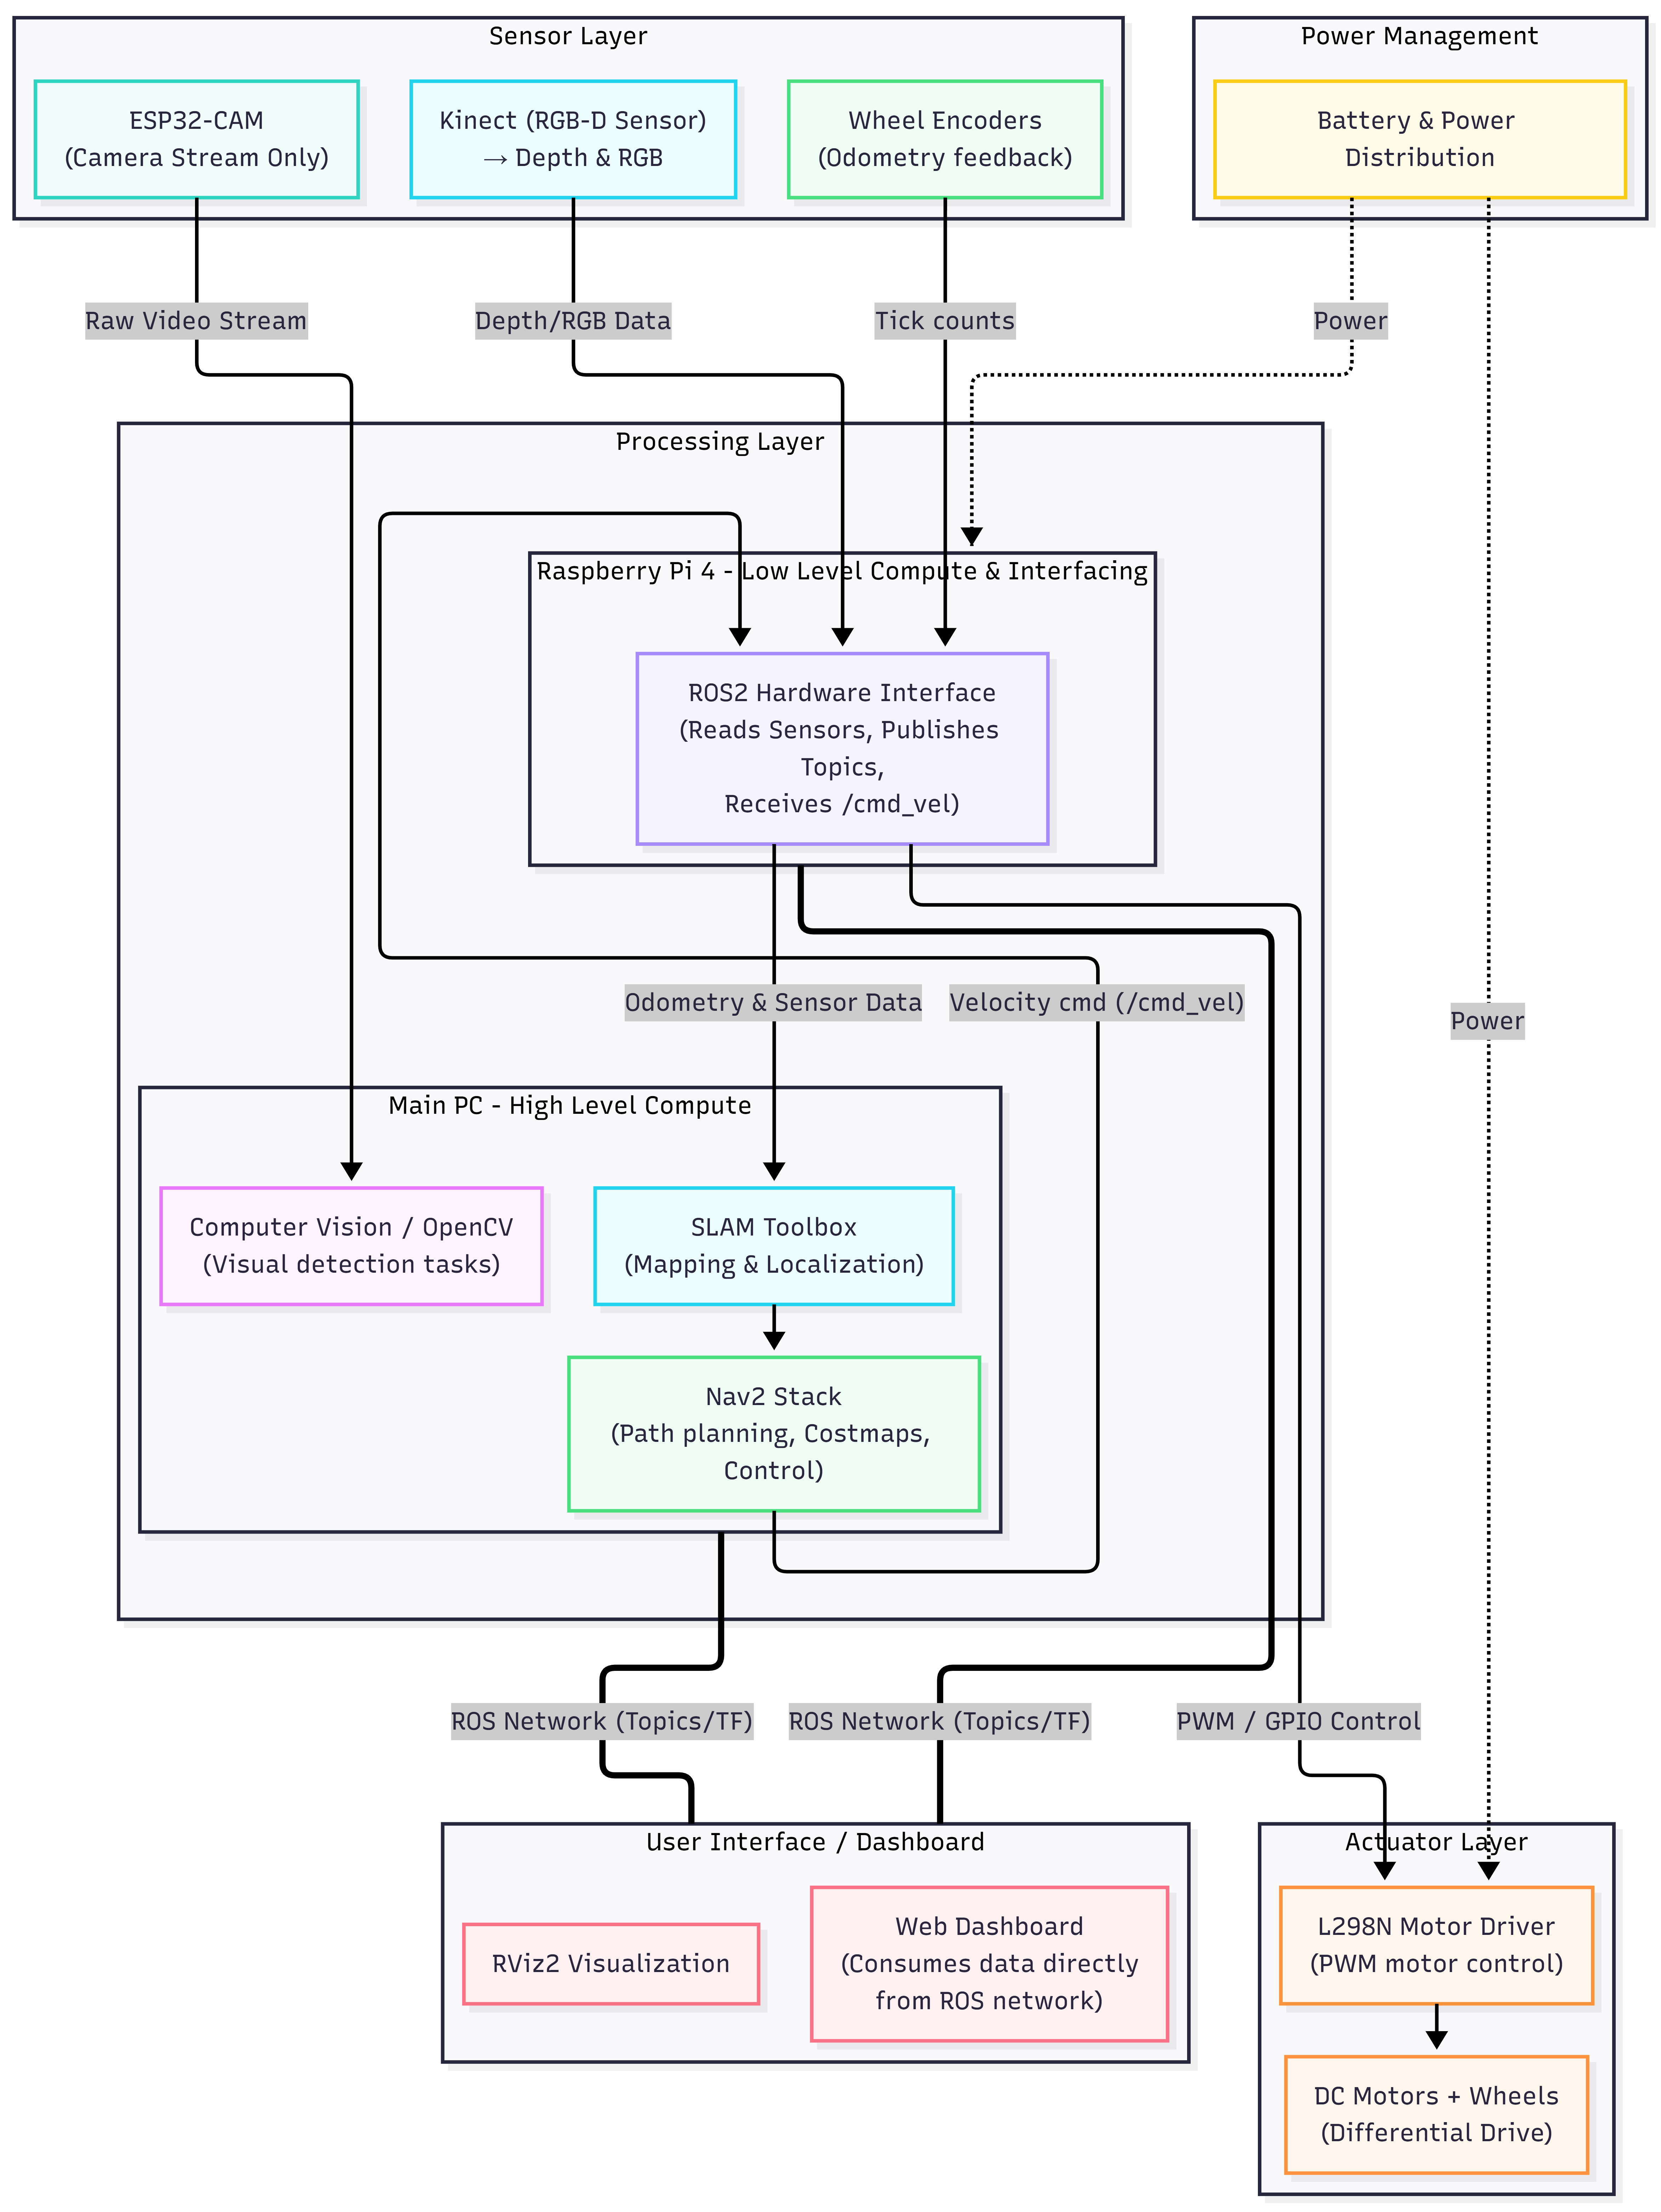
\includegraphics[width=0.62\linewidth]{images/Global_Archi.png}
	\caption{Architecture globale d'\esibot{} telle que construite (document fourni par
		l'équipe). Le capteur de cartographie principal est le Kinect (RGB-D) et non le
		radar ultrasonique du cahier des charges ; les moteurs sont pilotés directement
		par le Raspberry\,Pi\,4 et non par l'ESP32-CAM.}
	\label{fig:global_archi}
\end{figure}

Quatre observations structurantes ressortent de ce schéma et sont confirmées par le code
source~:

\begin{enumerate}
	\item \textbf{L'ESP32-CAM est réduit à une fonction unique de caméra de streaming.}
	      Le firmware \texttt{CameraServerArduinoIDE.ino} (variante du serveur de caméra
	      ESP32 standard d'Espressif, modèle \texttt{AI\_THINKER}) ne pilote ni moteurs, ni
	      servo, ni capteur de distance --- il expose uniquement un flux \gls{mjpeg} HTTP sur
	      le réseau \gls{wifi} local.
	\item \textbf{Le Raspberry\,Pi\,4 assure l'intégralité de l'interfaçage bas-niveau.} Le
	      nœud \texttt{motor\_bridge\_node} (paquet \texttt{esibot\_hardware}) pilote
	      directement le pont en H L298N et lit les encodeurs de roue via les broches
	      \gls{gpio} du Raspberry\,Pi --- une responsabilité initialement prévue pour
	      l'ESP32-CAM.
	\item \textbf{Le capteur de cartographie principal est un Kinect (v1), pas le radar
	      ultrasonique.} Le paquet \texttt{esibot\_slam} lance le pilote
	      \texttt{kinect\_ros2}, convertit son image de profondeur en balayage laser de
	      pseudo-portée via \texttt{depthimage\_to\_laserscan}, puis alimente
	      \texttt{slam\_toolbox}. Le nœud \texttt{ultrasonic\_scan\_node} existe toujours
	      dans le paquet \texttt{esibot\_sensors} mais son lancement est commenté dans le
	      script d'exploitation \texttt{start\_esibot\_all.sh} --- il s'agit donc d'un
	      chemin de code \emph{déprécié}, conservé mais non utilisé en exploitation
	      courante.
	\item \textbf{Une centrale inertielle (\gls{imu}) MPU6050} a été ajoutée, absente du
	      cahier des charges initial, et fusionnée à l'odométrie par encodeurs via un
	      filtre de Kalman étendu (\texttt{robot\_localization}), afin de stabiliser le cap
	      du robot et d'améliorer la précision de l'odométrie fournie à \gls{slam} et Nav2.
\end{enumerate}

\section{Découpage en trois couches}
\label{sec:archi_layers}

\paragraph{Couche 1 --- Capteurs (Sensor Layer).}
Trois sources de données indépendantes alimentent la couche de traitement~: l'ESP32-CAM
(flux vidéo brut \gls{mjpeg}), le Kinect (image de profondeur et image couleur RGB), et les
encodeurs de roue (comptage d'impulsions pour l'odométrie). Chaque source utilise une
interface physique distincte~: \gls{wifi} pour la caméra, USB pour le Kinect, \gls{gpio}
à interruption pour les encodeurs.

\paragraph{Couche 2 --- Traitement bas-niveau (Raspberry\,Pi\,4).}
Le Raspberry\,Pi\,4 héberge l'interface matérielle \ros{}\,2~: il lit les capteurs
embarqués (encodeurs, \gls{imu}), exécute la boucle d'asservissement de vitesse \gls{pid}
des deux moteurs, publie l'odométrie et les topics de télémétrie, et reçoit les commandes
de vitesse \topic{/cmd\_vel}.

\paragraph{Couche 3 --- Traitement haut-niveau (PC opérateur).}
Le schéma officiel positionne la vision par ordinateur (OpenCV), \pkg{slam\_toolbox} et la
pile Nav2 sur un PC principal distinct, communiquant avec le Raspberry\,Pi\,4 via le réseau
\ros{}\,2 (DDS, topics/\gls{tf}). Cette séparation logique est rendue possible par la
nature distribuée de \ros{}\,2~: les arguments de lancement
(\texttt{start\_base}, \texttt{start\_kinect}, \texttt{start\_slam}, \texttt{start\_rviz})
du fichier \texttt{mapping.launch.py} sont indépendamment activables, ce qui permet
d'exécuter les nœuds lourds (\gls{slam}, Nav2) sur une machine plus puissante que le
Raspberry\,Pi\,4 tout en laissant ce dernier dédié à l'interfaçage matériel temps-réel.

\paragraph{Couche transverse --- Alimentation.}
Une batterie et une distribution de puissance régulée alimentent indépendamment la couche
actionneurs (moteurs via L298N) et la couche de calcul (Raspberry\,Pi\,4, ESP32-CAM), comme
indiqué sur la figure~\ref{fig:global_archi}.

\section{Diagramme des nœuds et topics \ros{}\,2 réellement implémentés}
\label{sec:archi_nodes}

La figure~\ref{fig:ros_graph} reconstruit le graphe des nœuds et topics \emph{tel
qu'observable dans le code source actuel}, à distinguer du diagramme de flux
\emph{initialement prévu} par le cahier des charges (figure~\ref{fig:topics_stream_spec}),
qui mentionne des nœuds (\texttt{esibot\_driver}, \texttt{radar\_node},
\texttt{esircam\_node}, \texttt{vision\_node}, \texttt{web\_bridge}) dont les noms et,
pour certains, l'existence même, diffèrent de l'implémentation réelle. Cet écart est
analysé en détail au chapitre~\ref{ch:limitations}.

\begin{figure}[H]
	\centering
	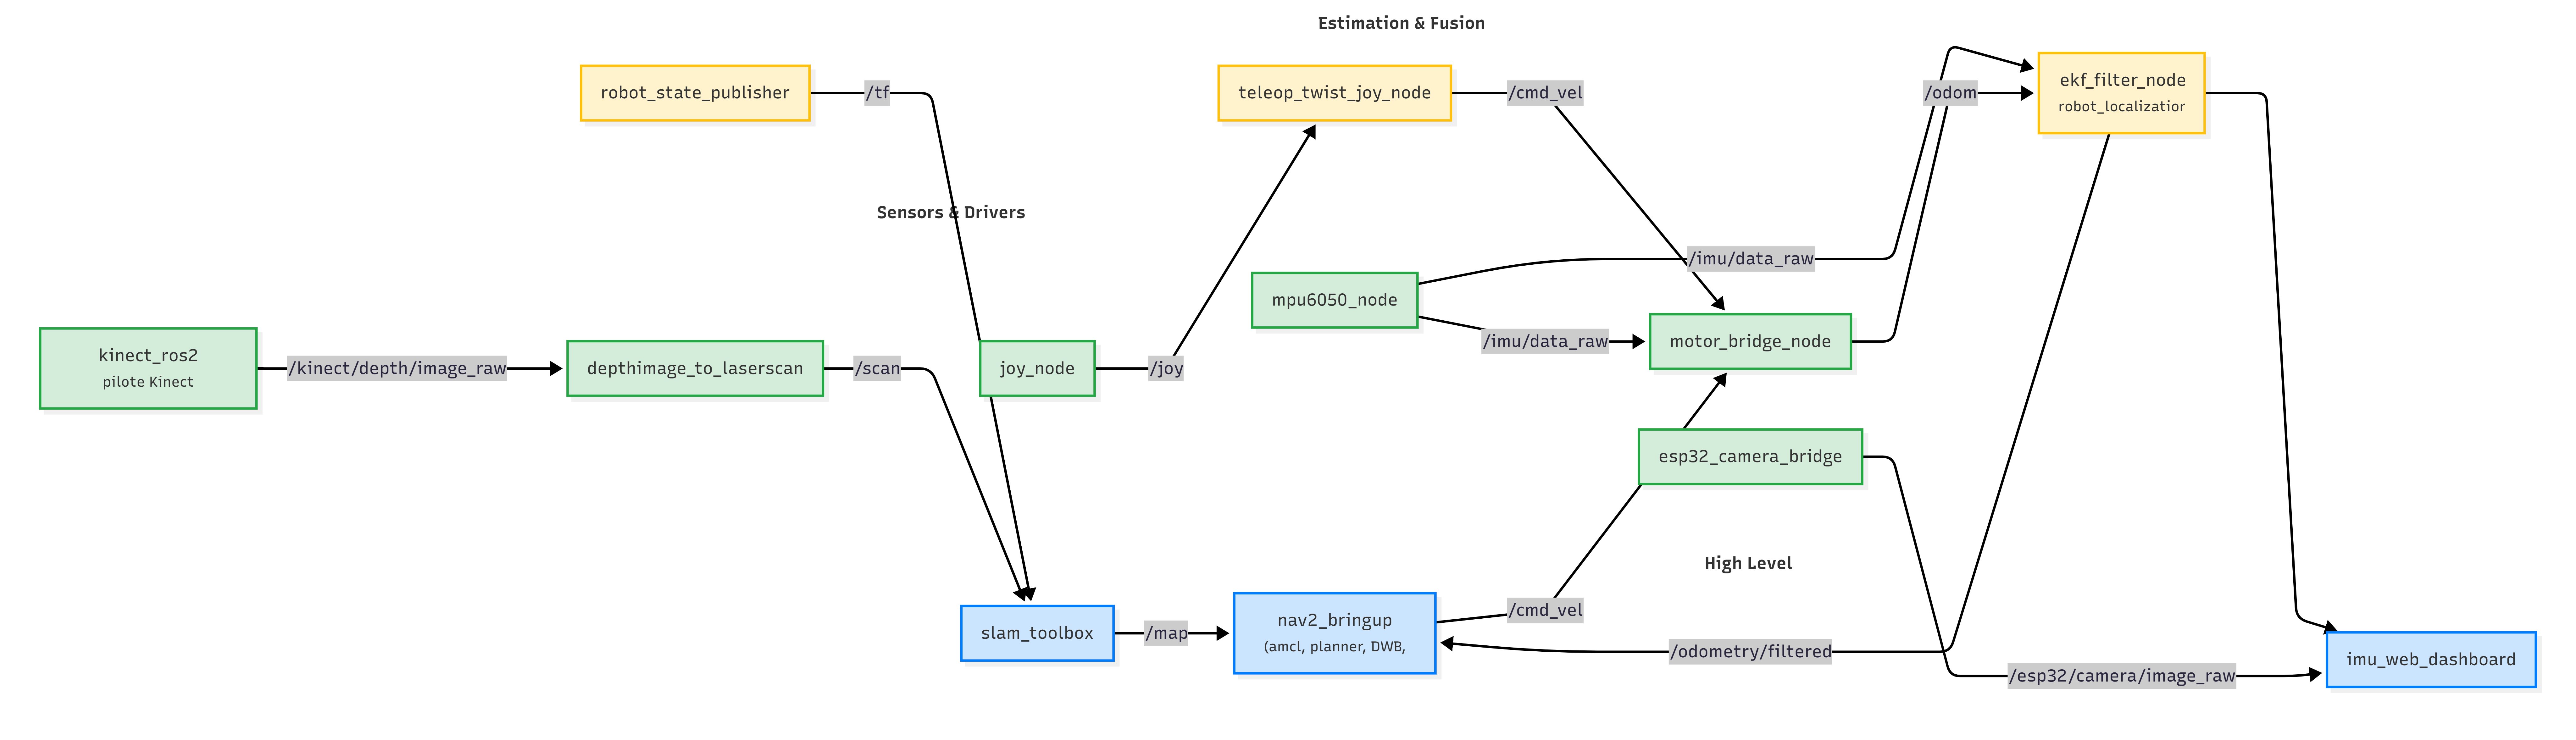
\includegraphics[width=0.78\linewidth]{images/Kinect_Stream.png}
	\caption{Graphe simplifié des noeuds et topics \ros{}\,2. Couleurs~: vert = pilotes capteurs/actionneurs,
		gris-bleu = estimation d'état, bleu = planification/cartographie haut-niveau.}
	\label{fig:topics_stream_spec}
\end{figure}

\section{Synthèse des topics principaux}
\label{sec:archi_topics_table}

Le tableau~\ref{tab:topics_summary} résume les topics \ros{}\,2 effectivement publiés ou
souscrits dans le code source. La liste exhaustive, avec types de message complets, est
fournie en annexe~\ref{app:topics}.

\begin{table}[H]
	\centering
	\caption{Topics \ros{}\,2 principaux --- architecture telle que construite.}
	\label{tab:topics_summary}
	\begin{tabularx}{\linewidth}{L{3.4cm} L{3.4cm} L{3.4cm} L{3.1cm}}
		\toprule
		\textbf{Topic} & \textbf{Type} & \textbf{Publié par} & \textbf{Souscrit par} \\
		\midrule
		\topic{/cmd\_vel} & geometry\_msgs/Twist & teleop\_twist\_joy, Nav2 & motor\_bridge\_node \\
		\topic{/odom} & nav\_msgs/Odometry & motor\_bridge\_node & ekf\_filter\_node \\
		\topic{/odometry/filtered} & nav\_msgs/Odometry & ekf\_filter\_node & Nav2, imu\_web\_dashboard \\
		\topic{/imu/data\_raw} & sensor\_msgs/Imu & mpu6050\_node & motor\_bridge\_node, ekf\_filter\_node, dashboard \\
		\topic{/scan} & sensor\_msgs/LaserScan & depthimage\_to\_laserscan (Kinect) & slam\_toolbox, Nav2 costmaps \\
		\topic{/map} & nav\_msgs/OccupancyGrid & slam\_toolbox & Nav2, \gls{rviz} \\
		\topic{/tf}, \topic{/tf\_static} & tf2\_msgs/TFMessage & robot\_state\_publisher, ekf, slam\_toolbox & Nav2, \gls{rviz} \\
		\topic{/joy} & sensor\_msgs/Joy & joy\_node & teleop\_twist\_joy\_node, dashboard \\
		\topic{/esp32/camera/image\_raw} & sensor\_msgs/Image & esp32\_camera\_bridge & (consommateur optionnel) \\
		\bottomrule
	\end{tabularx}
\end{table}

\chapter{Conception Mécanique et Électronique}
\label{ch:mecanique}

\section{Architecture différentielle}
\label{sec:meca_diff}

\esibot{} adopte une architecture \emph{differential drive}~: deux roues motrices
indépendantes plus une roue folle assurant la stabilité statique, la direction résultant
uniquement de la différence de vitesse entre les deux roues. Les fichiers \gls{cad}/STL du
châssis constituent un livrable séparé (Livrable~1) non inclus dans le code analysé~; ce
chapitre s'appuie donc sur le modèle \gls{urdf} (\texttt{esibot\_description}), source de
vérité utilisée par \ros{} pour les transformées et les costmaps, complété par les
constantes électroniques relevées dans le code de commande.

\section{Modèle géométrique}
\label{sec:meca_urdf}

\begin{table}[H]
	\centering
	\caption{Paramètres géométriques et inertiels déclarés dans le modèle \gls{urdf}.}
	\label{tab:urdf_geom}
	\begin{tabularx}{\linewidth}{L{5cm} C{3.2cm} L{5cm}}
		\toprule
		\textbf{Élément} & \textbf{Valeur} & \textbf{Remarque} \\
		\midrule
		Châssis (\texttt{base\_link}) & 0.21 $\times$ 0.14 $\times$ 0.03\,m & masse 2.0\,kg \\
		Rayon de roue (\texttt{wheel\_radius}) & 0.025\,m & largeur 0.027\,m, masse 0.2\,kg/roue \\
		Empattement (\texttt{wheel\_y} $\times 2$) & 0.14\,m & distance latérale entre roues \\
		Module caméra (\texttt{camera\_link}) & 0.073 $\times$ 0.278 $\times$ 0.073\,m & masse 0.56\,kg, $x=-0.105$\,m (arrière) \\
		\bottomrule
	\end{tabularx}
\end{table}

Le modèle déclare les repères optiques caméra (\texttt{camera\_depth\_frame},
\texttt{camera\_rgb\_optical\_frame}, rotation $-\pi/2$) ; un
\texttt{static\_transform\_publisher} relie \texttt{camera\_depth\_frame} au repère natif
du pilote Kinect \texttt{kinect\_depth} par une transformée identité.

\begin{warnbox}
	Une révision des paramètres géométriques (notamment le rayon des roues et l'empattement) est nécessaire pour garantir une parfaite cohérence entre le modèle \gls{urdf} et le code de commande bas-niveau, afin d'optimiser la précision de l'odométrie.
\end{warnbox}

\section{Cinématique différentielle et odométrie}
\label{sec:meca_kinematics}

La conversion \topic{/cmd\_vel} $\to$ vitesses de roue, implémentée dans
\texttt{motor\_bridge\_node.py} (\texttt{twist\_to\_wheel\_\allowbreak commands}) et répliquée dans le
tableau de bord (\texttt{imu\_web\_dashboard.py}), suit le modèle classique~:

\begin{equation}
	v_{\text{g}} = v - \omega \cdot \tfrac{L}{2}, \quad
	v_{\text{d}} = v + \omega \cdot \tfrac{L}{2}
	\label{eq:diff_drive}
\end{equation}

et inversement pour la reconstruction d'odométrie~:
$v = (v_{\text{g}}+v_{\text{d}})/2$, $\omega = (v_{\text{d}}-v_{\text{g}})/L$
(équation~\ref{eq:diff_drive_inverse}), où $L$ est l'empattement.
\begin{equation}
	v = \frac{v_{\text{g}} + v_{\text{d}}}{2}, \qquad
	\omega = \frac{v_{\text{d}} - v_{\text{g}}}{L}
	\label{eq:diff_drive_inverse}
\end{equation}

\begin{figure}[H]
	\centering
	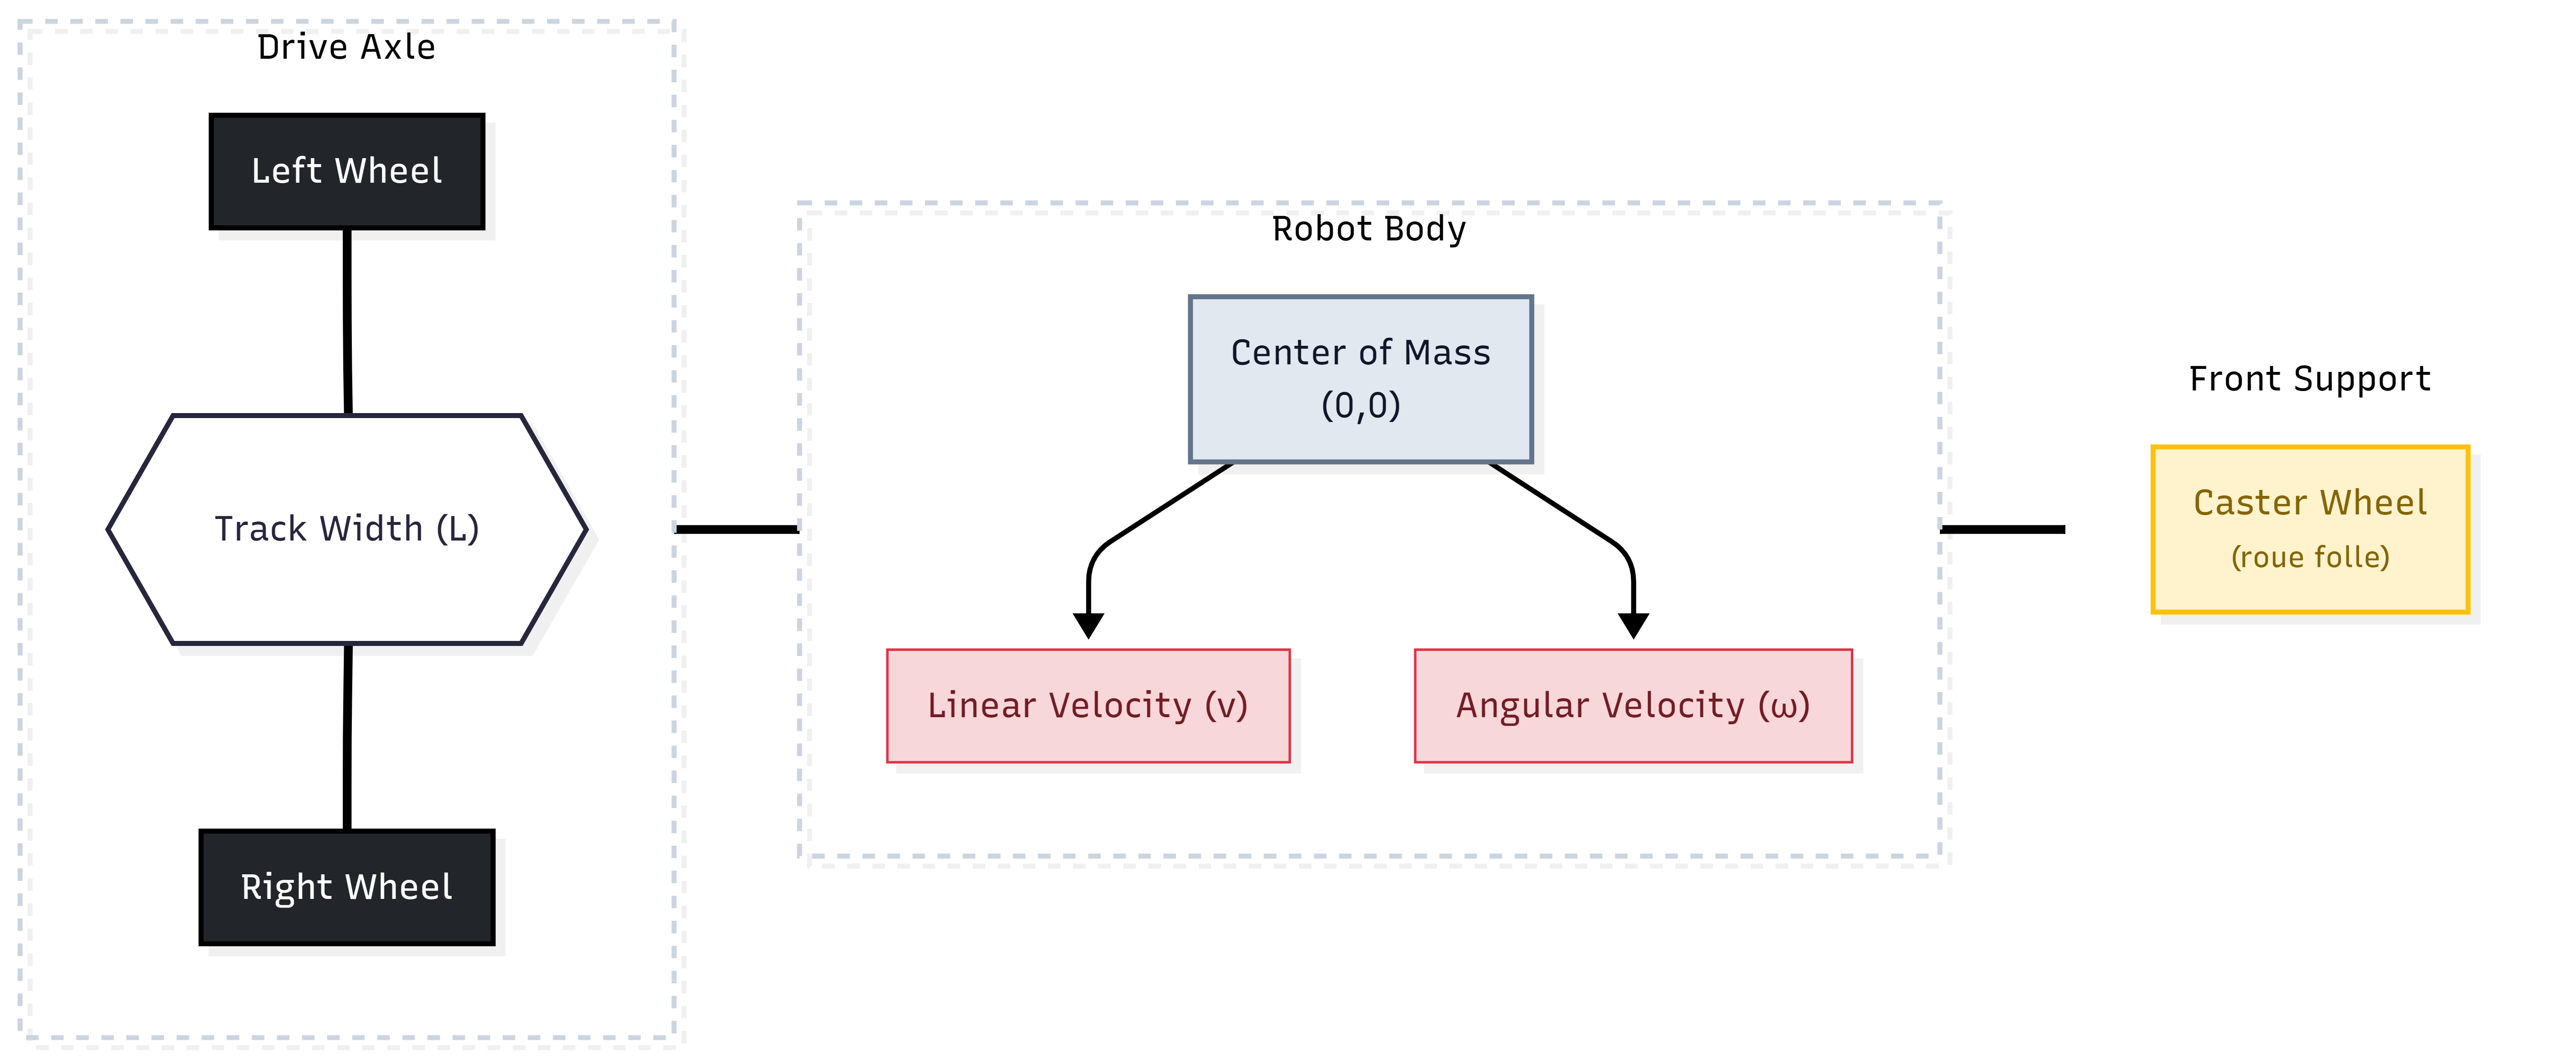
\includegraphics[width=0.5\linewidth]{images/diff_drive_diagram.png}
	\caption{Modèle cinématique du robot différentiel \esibot{} (vue de dessus).}
	\label{fig:diff_drive_diagram}
\end{figure}

Chaque roue est équipée d'un encodeur compté par interruption \gls{gpio}, anti-rebond
logiciel 2\,ms. Le paramètre \texttt{encoder\_cpr} (12 par défaut) est doublé par comptage
sur les deux fronts (\texttt{encoder\_count\_both\_\allowbreak edges=True}), donnant
\textbf{24 impulsions/tour}. La vitesse de rotation mesurée est calculée à chaque cycle de
contrôle (\texttt{control\_hz}, 10\,Hz par défaut) par~:
\begin{equation}
	\text{RPM}_{\text{mesuré}} = \frac{N_{\text{impulsions}}}{\text{CPR}_{\text{effectif}}} \times \frac{60}{\Delta t}
	\label{eq:rpm_measure}
\end{equation}
soit $360^\circ/24=15^\circ$ par impulsion et, avec le rayon de 0.033\,m du calibrateur,
$\approx$\textbf{8.6\,mm}/impulsion ($2\pi\times0.033/24$).

\section{Câblage électronique}
\label{ch:electronique}
\label{sec:elec_topology}

Le cahier des charges (Livrable~2) exige un schéma Fritzing/KiCad, absent de l'archive
fournie~; le tableau~\ref{tab:gpio_pinout} a donc été \textbf{reconstruit par
rétro-ingénierie} depuis les constantes \gls{gpio} du code Python. À la différence du
cahier des charges, qui prévoyait que l'ESP32-CAM pilote le pont en H, le servo et le
HC-SR04, l'implémentation réelle concentre toute l'électronique temps-réel sur les broches
\gls{gpio} du Raspberry\,Pi\,4.

\begin{table}[H]
	\centering
	\caption{Broches \gls{gpio} du Raspberry\,Pi\,4 (BCM), reconstruites depuis le code source.}
	\label{tab:gpio_pinout}
	\begin{tabularx}{\linewidth}{L{3.8cm} C{1.6cm} L{6.8cm}}
		\toprule
		\textbf{Fonction} & \textbf{GPIO} & \textbf{Source / nœud} \\
		\midrule
		ENA / IN1 / IN2 (moteur g.) & 12 / 5 / 6 & \texttt{motor\_bridge\_node}, \texttt{motor\_calibrator} \\
		Encodeur gauche & 26 & \texttt{motor\_bridge\_node} (\texttt{pin\_left\_encoder}) \\
		ENB / IN3 / IN4 (moteur d.) & 13 / 21 / 20 & \texttt{motor\_bridge\_node}, \texttt{motor\_calibrator} \\
		Encodeur droit & 27 & \texttt{motor\_bridge\_node} (\texttt{pin\_right\_encoder}) \\
		\gls{i2c} SDA/SCL (bus 1) & 2 / 3 & \texttt{mpu6050\_node} (MPU6050 @ 0x68) \\
		HC-SR04 SIG (trig/écho) & 23 & \texttt{ultrasonic\_scan\_node} (déprécié) \\
		Servo SG90 radar & 18 & \texttt{ultrasonic\_scan\_node} (déprécié) \\
		\bottomrule
	\end{tabularx}
\end{table}

Dans la branche \texttt{working\_build}, le câblage logiciel du calibrateur et celui du
nœud de production sont cohérents~: les deux utilisent les broches BCM~26 et BCM~27 pour
les encodeurs gauche et droit. La calibration PWM$\to$RPM peut donc alimenter directement
\texttt{pwm\_mapper.py}, sous réserve que le rayon de roue et l'empattement utilisés par
l'odométrie soient contrôlés expérimentalement (voir chapitre~\ref{ch:limitations}).

Le pilotage moteur utilise un double pont en H \textbf{L298N} en PWM logiciel
(\texttt{RPi.GPIO}, 500\,Hz), rapport cyclique borné à $[15\,\%,100\,\%]$
(\texttt{min/max\_duty\_cycle}) pour compenser la zone morte mécanique. Le MPU6050
(\gls{i2c} bus~1, adresse \texttt{0x68}) est configuré au démarrage (réveil, diviseur
d'échantillonnage \texttt{SMPLRT\_DIV=0x07}, filtre passe-bas \texttt{DLPF\_CFG=0x03},
$\pm2g$/$\pm250^\circ$/s) et publie à \textbf{50\,Hz}. Le Kinect (v1, ère Xbox\,360), capteur de
cartographie principal, est relié en \textbf{USB} (non \gls{gpio}) et piloté par le paquet
communautaire \texttt{kinect\_ros2} (\texttt{libfreenect}).

\section{Serveur de caméra (ESP32-CAM)}
\label{sec:elec_esp32cam}

Le module ESP32-CAM (\texttt{AI\_THINKER}) sert exclusivement de serveur vidéo \gls{mjpeg}
\gls{wifi}~: le firmware \texttt{CameraServerArduinoIDE.ino} initialise le capteur OV2640
(\texttt{UXGA} si PSRAM, sinon \texttt{SVGA}) et expose le flux sur \texttt{/stream}.
Aucune broche \gls{gpio} de l'ESP32-CAM ne pilote d'actionneur --- l'essentiel de ses
broches étant réservé à l'interface caméra parallèle --- une contrainte matérielle
probablement à l'origine du report de la commande moteur vers le Raspberry\,Pi\,4. Les
identifiants \gls{wifi} (SSID/mot de passe) sont \textbf{codés en dur} dans le firmware,
sans portail captif ni provisioning (chapitre~\ref{ch:limitations}).

\section{Alimentation}
\label{sec:elec_power}

Le schéma d'architecture (figure~\ref{fig:global_archi}) identifie un bloc « Power
Management » alimentant séparément la couche actionneurs (L298N) et la couche de calcul
(Raspberry\,Pi\,4, ESP32-CAM). Aucun nœud de supervision de batterie
(\topic{/battery\_state}, prévu au cahier des charges) n'a été retrouvé dans le code~: la
télémétrie de batterie n'est, à ce stade, pas exposée par le logiciel embarqué.

\chapter{Low-Level Control and Sensor Fusion}
\label{ch:commande_bas_niveau}

\section{Motor Control (\texttt{motor\_bridge\_node})}
\label{sec:cbn_motor_bridge}

This node (package \texttt{esibot\_hardware}) is the core of the robot's real-time
control. On the Raspberry\,Pi\,4, it plays the role originally assigned to the
ESP32/\texttt{esibot\_driver} pair in the specification: receiving \topic{/cmd\_vel},
wheel velocity control, encoder reading, and publishing raw odometry.

\subsection{Control Loop}
\label{sec:cbn_loop}

The node runs a periodic loop at \texttt{control\_hz} (10\,Hz by default) which, on each
cycle:
\begin{enumerate}
	\item reads the pulse counts accumulated since the last cycle for each wheel;
	\item computes the measured rotation speed in \unit{\rpm} (equation~\ref{eq:rpm_measure});
	\item applies a \gls{pid} controller (one per wheel) to bring the measured speed closer to
	      the setpoint derived from the differential kinematics (equation~\ref{eq:diff_drive});
	\item converts the controller output into a PWM duty cycle via \texttt{pwm\_mapper.py};
	\item applies an optional heading correction based on the \gls{imu} (yaw control);
	\item publishes the integrated odometry on \topic{/odom} and the counter status on the
	      diagnostic topics (\topic{/encoder\_ticks\allowbreak/left}, \topic{/encoder\_ticks\allowbreak/right}).
\end{enumerate}

\subsection{Per-Wheel \gls{pid} Controller}
\label{sec:cbn_pid}

Each wheel has its own independent \gls{pid} controller, with default gains $K_p$,
$K_i$, $K_d$ configurable via the \ros{} parameter server (and adjustable during
operation without recompilation). The controller output is saturated, and an
anti-\emph{windup} mechanism limits accumulation of the integral term when the command is
saturated, avoiding overshoot during abrupt setpoint changes.

\begin{notebox}[title={Safety Loop}]
	The node implements a \emph{watchdog} timer: if no \topic{/cmd\_vel} message is
	received for a duration \texttt{cmd\_vel\_timeout} (typically a few hundred
	milliseconds), both motors are automatically cut off. This mechanism protects the
	robot in case of network communication loss with the teleoperation node or Nav2.
\end{notebox}

\section{Wheel Speed to PWM Conversion}
\label{sec:cbn_pwm_mapper}

The \texttt{pwm\_mapper.py} module converts a desired linear wheel speed (in
\unit{\metre\per\second}) into a normalized PWM duty cycle. In \texttt{working\_build},
this conversion is no longer a simple theoretical calibration: it loads the
\texttt{\textasciitilde/.esibot/pwm\_rpm\_map.json} file, generated on the robot, and
applies a separate affine regression for each wheel and direction of travel. The
conversion combines:
\begin{itemize}
	\item a mechanical dead zone (\texttt{min\_duty\_cycle}, 15\,\% by default and 22\,\%
	      in some launches without calibration);
	\item \texttt{a}/\texttt{b} coefficients calibrated for \texttt{left/right} and
	      \texttt{forward/reverse}, to compensate for efficiency differences between the
	      two motors;
	\item a cap at \texttt{max\_pwm}/\texttt{max\_rpm} derived from calibration, which
	      avoids commanding into a saturation or mechanical-noise region.
\end{itemize}

\section{Calibration Tool (\texttt{motor\_calibrator.py})}
\label{sec:cbn_calibrator}

A standalone calibration script (outside the \ros{} graph, run from the command line)
empirically characterizes the relationship between PWM duty cycle and actual rotation
speed (in \unit{\rpm}) for each motor. It sweeps duty cycles from 15\,\% to 100\,\% in
5\,\% steps, measures two one-second samples per point, keeps the median, then stops the
sweep as soon as an RPM drop indicates saturation or an unstable reading. The result is
saved to \texttt{\textasciitilde/.esibot/pwm\_rpm\_map.json} along with the wheel radius
used (0.033\,m), the PWM frequency (500\,Hz) and the forward/reverse coefficients for
each wheel. This tool is essential for limiting motor mechanical asymmetry, but it alone
is not sufficient to guarantee correct odometry if the actual wheel radius, wheelbase and
\gls{slam} parameters are not recalibrated together (Chapter~\ref{ch:limitations}).

\section{Inertial Measurement Unit and Heading Stabilization}
\label{sec:cbn_imu}

The \texttt{mpu6050\_node} node (package \texttt{esibot\_sensors}) starts with a
stationary gyroscope bias calibration over 100 samples, then continuously publishes
(50\,Hz):
\begin{itemize}
	\item \topic{/imu/data\_raw} (\texttt{sensor\_msgs/Imu}) --- raw linear accelerations
	      $(a_x, a_y, a_z)$ and angular velocities $(\omega_x, \omega_y, \omega_z)$;
	\item \topic{/imu/temperature} (\texttt{sensor\_msgs/Temperature}) --- internal sensor
	      temperature, useful for thermal diagnostics.
\end{itemize}

\texttt{motor\_bridge\_node} subscribes to \topic{/imu/data\_raw} to apply closed-loop
yaw correction when the robot is moving forward and no deliberate rotation is commanded.
The controller compensates for residual yaw rate measured by the \gls{imu}, with a dead
band of 0.02\,rad/s and a maximum correction of 40\,RPM per wheel.

\section{Data Fusion (EKF Filter)}
\label{sec:cbn_ekf}

Raw odometry (\topic{/odom}, from encoders alone) and inertial data
(\topic{/imu/data\_raw}) are fused by an \gls{ekf} provided by the standard
\texttt{robot\_localization} package (\texttt{ekf\_filter\_node} node), configured in
two-dimensional mode (\texttt{two\_d\_mode: true}). The \texttt{working\_build}
\texttt{ekf\_odom\_imu.yaml} file is deliberately conservative: it fuses the odometry
velocities $(v_x,v_y,\dot\theta)$ and only the yaw rate from the \gls{imu}. It injects
neither absolute orientation nor linear acceleration, since the MPU6050 does not publish
an estimated orientation and its raw acceleration contains gravity and residual bias.
The \topic{/odometry/filtered} output thus provides a more stable local odometry for
\gls{slam}/Nav2, while \texttt{slam\_toolbox} or \gls{amcl} retain responsibility for the
global \topic{map}~$\rightarrow$~\topic{odom} correction.

\chapter{Mapping and Autonomous Navigation}
\label{ch:slam}

\section{Kinect to \gls{slam} Pipeline}
\label{sec:slam_overview}

The system relies on a \textbf{Kinect} depth sensor to generate the environment map.
The extracted depth data is converted into a 2D laser scan. This approach provides the
standard \texttt{sensor\_msgs/LaserScan} message structure expected by the \gls{slam}
algorithm. The \texttt{mapping.launch.py} file launches and orchestrates this entire
chain (Figure~\ref{fig:slam_pipeline}).

\begin{figure}[H]
	\centering
	\resizebox{0.92\linewidth}{!}{%
		\begin{tikzpicture}[
				stage/.style={draw, rounded corners=4pt, minimum height=1.1cm, minimum width=2.7cm,
						fill=EsiGray, font=\scriptsize\bfseries, text=EsiDark, align=center},
				arr/.style={-Stealth, thick, EsiBlue!80},
				lbl/.style={font=\tiny, text=EsiAccent, align=center}
			]
			\node[stage, fill=EsiGreen!15] (kinect) at (0,0) {Kinect (v1)\\\tiny RGB-D sensor};
			\node[stage, fill=EsiGreen!15] (driver) at (3.4,0) {kinect\_ros2\_node\\\tiny libfreenect driver};
			\node[stage, fill=EsiAccent!18] (d2l) at (7.0,0) {depthimage\_to\_\\laserscan\_node};
			\node[stage, fill=EsiBlue!15] (slam) at (10.6,0) {async\_slam\_\\toolbox\_node};
			\node[stage, fill=EsiBlue!15] (rviz) at (10.6,-2.1) {\gls{rviz} 2\\\tiny visualization};

			\draw[arr] (kinect) -- node[lbl, above]{USB} (driver);
			\draw[arr] (driver) -- node[lbl, above]{/kinect/depth/\\image\_raw} (d2l);
			\draw[arr] (d2l) -- node[lbl, above]{/scan\\(LaserScan)} (slam);
			\draw[arr] (slam) -- node[lbl, right]{/map} (rviz);
			\draw[arr] (slam.south) -- ++(0,-0.7) -| node[lbl, pos=0.25, above]{/tf (map$\to$odom)} (rviz.north);
		\end{tikzpicture}
	}
	\caption{Mapping pipeline as orchestrated by \texttt{mapping.launch.py}.}
	\label{fig:slam_pipeline}
\end{figure}

The \texttt{kinect\_ros2} driver (namespace \texttt{kinect}, based on
\texttt{libfreenect}) exposes \topic{/kinect/depth/image\_raw} and
\topic{/kinect/depth/camera\_info}. A \texttt{static\_transform\_publisher} links
\texttt{camera\_depth\_frame} (\gls{urdf}) to the native \texttt{kinect\_depth} frame via
an identity transform. The \texttt{depthimage\_to\_laserscan\_node}
\label{sec:slam_d2l}
node then
projects a horizontal band of the depth image into a synthetic laser scan
(Table~\ref{tab:d2l_params}).

\begin{table}[H]
	\centering
	\caption{Parameters of \texttt{depthimage\_to\_laserscan\_node} (\texttt{mapping.launch.py}).}
	\label{tab:d2l_params}
	\begin{tabularx}{\linewidth}{L{4cm} C{2.4cm} L{6.2cm}}
		\toprule
		\textbf{Parameter} & \textbf{Value} & \textbf{Meaning} \\
		\midrule
		\texttt{scan\_height} & 10\,px & band of the depth image averaged per scan \\
		\texttt{scan\_time} & 0.033\,s & nominal period ($\approx$30\,Hz) \\
		\texttt{range\_min} / \texttt{max} & 0.35 / 4.0\,m & usable Kinect range \\
		\texttt{output\_frame} & \texttt{camera\_depth\_frame} & \gls{tf} frame of the \texttt{LaserScan} \\
		\bottomrule
	\end{tabularx}
\end{table}

\begin{notebox}[title={Reduced Field of View}]
	The Kinect covers $\approx57^\circ$ horizontally compared with the 180--360 degrees
	planned for a rotating radar or a panoramic LiDAR: the lateral/rear zones remain
	blind at any given instant, requiring active rotation of the robot during mapping to
	compensate.
\end{notebox}

\section{Depth Preprocessing with \texttt{depth\_cleanup}}
\label{sec:slam_depth_cleanup}

The \texttt{working\_build} branch adds the \texttt{depth\_cleanup} package (C++/OpenCV, independent of \ros{}/\texttt{libfreenect}) to fill holes in the Kinect depth data while preserving a metric \texttt{CV\_16UC1} image in millimeters. The \texttt{applyKinectSmoothingPipeline()} function: treats null pixels as invalid; fills small holes with a $3\times3$ mode filter (10\,mm bins); fills remaining holes with \texttt{cv::INPAINT\_TELEA} at 20\,\% resolution to limit CPU cost; and leaves original valid pixels unchanged. The remaining integration step is inserting a \ros{} adapter to publish the cleaned image and remap \texttt{depthimage\_to\_laserscan} to it, rather than \topic{/kinect/depth/image\_raw}.

\section{Why the Kinect Replaces the Ultrasonic Radar}
\label{sec:slam_ultrasonic_vs_kinect}

The \texttt{working\_build} ultrasonic path sweeps $-30^\circ$ to $+30^\circ$ in $5^\circ$ steps, waits 0.35\,s for servo settling, and publishes $\approx$0.07\,scans/s --- making it unsuitable for real-time mapping and easily confused by chairs, table legs, or sloped surfaces. The Gazebo simulation (Section~\ref{sec:slam_gazebo_sim}) confirmed these limits. The Kinect instead extracts a coherent \texttt{LaserScan} slice from a depth scene updated at video rate, feeding \texttt{slam\_toolbox}, Nav2 and autonomous exploration. The ultrasonic radar retains value only as a diagnostic tool or local safety check.

\section{\texttt{slam\_toolbox} Configuration}
\label{sec:slam_toolbox_config}

\texttt{slam\_toolbox\_esibot\_kinect.yaml} configures \texttt{async\_slam\_toolbox\_node}
in \texttt{mapping} mode (Ceres solver, \texttt{SPARSE\_NORMAL\_CHOLESKY}).
Table~\ref{tab:slam_params} summarizes the key parameters.

\begin{table}[H]
	\centering
	\caption{Key \texttt{slam\_toolbox} parameters for \esibot{}.}
	\label{tab:slam_params}
	\begin{tabularx}{\linewidth}{L{5cm} C{2.4cm} L{5cm}}
		\toprule
		\textbf{Parameter} & \textbf{Value} & \textbf{Role} \\
		\midrule
		\texttt{resolution} & 0.05\,m & cell size of the occupancy grid \\
		\texttt{min/max\_laser\_range} & 0.35 / 4.0\,m & consistent with \texttt{depthimage\_to\_laserscan} \\
		\texttt{minimum\_time\_interval} & 0.5\,s & minimum interval between processed scans \\
		\texttt{minimum\_travel\_distance/heading} & 0.15\,m / 0.15\,rad & anti-oversampling filter \\
		\texttt{do\_loop\_closing} & \texttt{true} & loop closure enabled (radius 3.0\,m) \\
		\texttt{transform\_publish\_period} & 0.02\,s & \topic{map}$\to$\topic{odom} publication ($\approx$50\,Hz) \\
		\bottomrule
	\end{tabularx}
\end{table}

\texttt{use\_map\_saver: true} enables on-demand saving
(\texttt{map\_saver\_cli}) as a \texttt{map.pgm}/\texttt{map.yaml} pair, subsequently
consumed by Nav2.

\begin{warnbox}
	\label{sec:slam_map_state}
	The current map used by \texttt{esibot\_navigation2} (resolution 0.05\,m, origin
	$(-10,-10,0)$) corresponds, upon visual inspection, to the default TurtleBot3/Nav2
	sample hexagonal map, and not to an actual map captured by \esibot{}'s Kinect. The
	\gls{slam}~$\to$~save~$\to$~Nav2 reload chain therefore still needed field
	validation at the time of writing (Chapter~\ref{ch:resultats}).
\end{warnbox}

The \gls{rviz} configuration \texttt{esibot\_slam\_map\allowbreak.rviz} is the project's
main visualization tool (map, \topic{/scan} scan, \gls{urdf} model, full \gls{tf} tree),
rather than an integrated mapping view in the web dashboard (Chapter~\ref{ch:ihm}).

\section{Gazebo Ultrasonic SLAM Simulation}
\label{sec:slam_gazebo_sim}

Before deploying on the physical robot, the ultrasonic-based occupancy grid algorithm was validated in a Gazebo simulation environment (\texttt{ultrasonic\_slam\_simulation} branch). The node \texttt{occupancy\_grid\_hcsr04} subscribes to \topic{/scan} (a simulated \texttt{LaserScan} from the virtual HC-SR04 array), runs a Bayesian log-odds update ($\text{log-odds}_{\text{free}}=-0.7$, $\text{log-odds}_{\text{occ}}=+1.5$, clipped to $[\,-3.0,\,3.0\,]$) on a $200\times200$ grid at 5\,cm/cell, and publishes both an \texttt{OccupancyGrid} on \topic{/map} and a \texttt{PointCloud2} on \topic{/map\_points} (workaround for an Nvidia display issue with RViz2).

\begin{figure}[H]
	\centering
	\begin{minipage}[b]{0.31\linewidth}
		\centering
		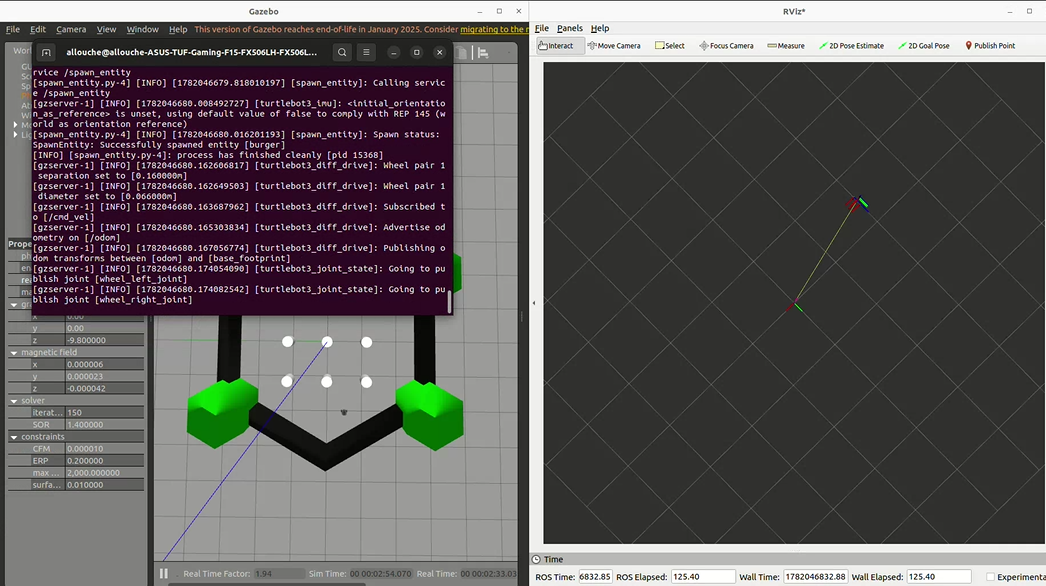
\includegraphics[width=\linewidth,height=4cm,keepaspectratio]{images/GazeboUltraSoundSimulationStartup.png}
		\caption*{\small (a) Startup.}
	\end{minipage}\hfill
	\begin{minipage}[b]{0.31\linewidth}
		\centering
		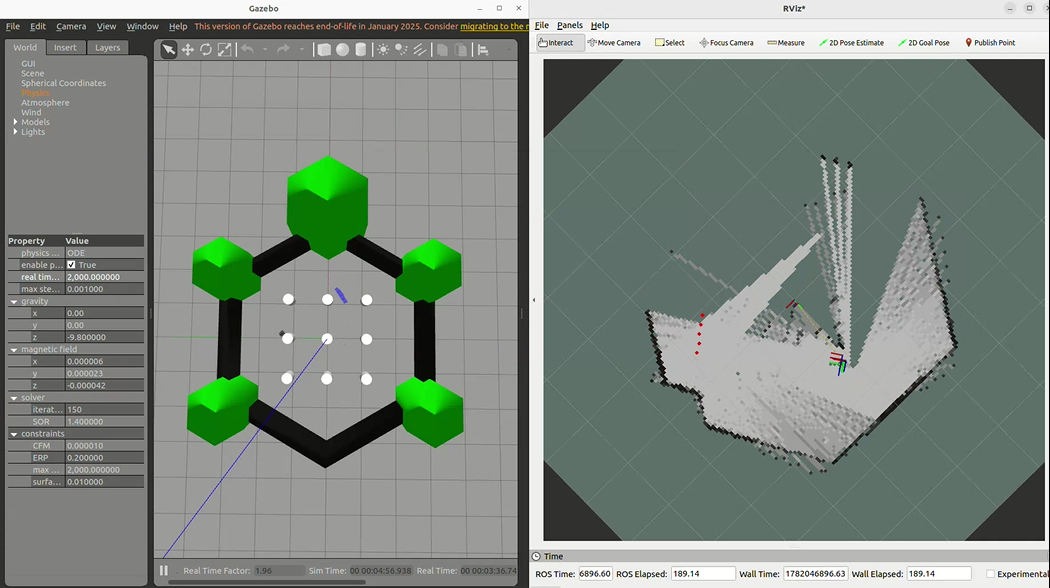
\includegraphics[width=\linewidth,height=4cm,keepaspectratio]{images/GazeboUltraSoundSimulationHalfProgress.png}
		\caption*{\small (b) Mid-exploration.}
	\end{minipage}\hfill
	\begin{minipage}[b]{0.31\linewidth}
		\centering
		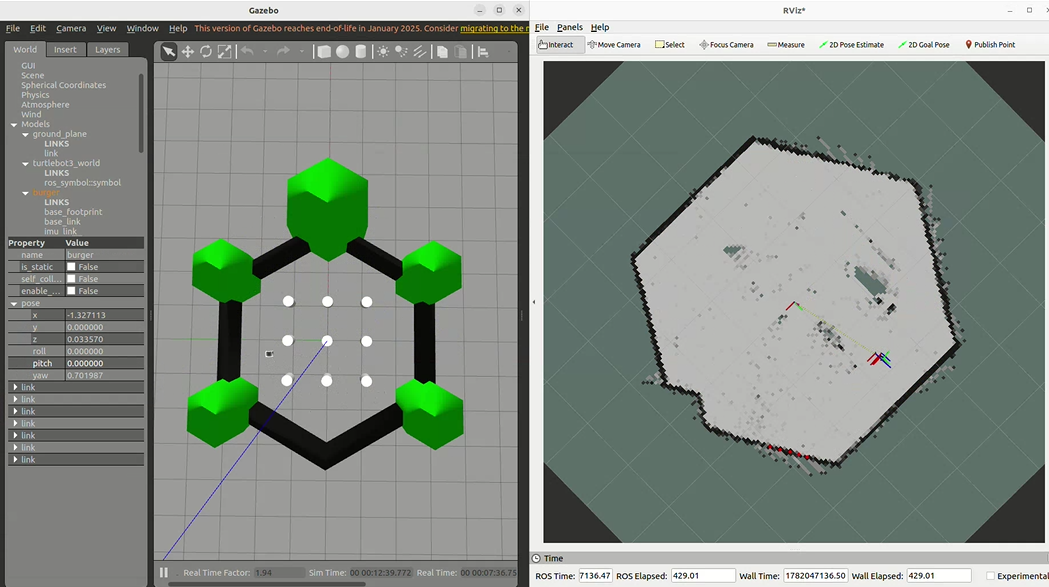
\includegraphics[width=\linewidth,height=4cm,keepaspectratio]{images/GazeboUltraSoundSimulationFinal.png}
		\caption*{\small (c) Final map.}
	\end{minipage}
	\caption{Gazebo simulation of ultrasonic occupancy-grid mapping (\texttt{ultrasonic\_slam\_simulation} branch). The robot autonomously explores a hexagonal arena using a AVANCER / EVITER / TOURNER state machine.}
	\label{fig:gazebo_ultrasound}
\end{figure}

The autonomous navigation relies on a three-state machine: \texttt{AVANCER} (forward at 0.07\,m/s), \texttt{EVITER} (obstacle avoidance at $<$0.85\,m), and \texttt{TOURNER} (rotation at $\pm$0.45\,rad/s). The Bayesian update runs at 20\,Hz (50\,ms timer), while the grid is published at 1\,Hz with Nav2-compatible QoS (\texttt{TRANSIENT\_LOCAL} + \texttt{RELIABLE}). As confirmed in Section~\ref{sec:slam_ultrasonic_vs_kinect}, this simulation demonstrated the limits of the slow ultrasonic sweep for real-time mapping, motivating the switch to the Kinect.

\section{Autonomous Navigation with Nav2}
\label{ch:navigation}

Autonomous navigation relies on the standard \textbf{Nav2} stack
(\texttt{navigation2.launch.py}, package \texttt{esibot\_navigation2}), loading the
static map, \texttt{esibot.yaml}, and orchestrating \gls{amcl} localization (500--2000 particles,
\texttt{likelihood\_field} + \texttt{DifferentialMotionModel}), costmaps, planner, controller,
velocity smoother and collision monitor. Local and global costmaps
\label{sec:nav_costmaps}
share 0.05\,m/cell resolution, 0.2\,m robot radius, 0.35\,m inflation radius.
\texttt{NavfnPlanner} (Dijkstra, 0.5\,m tolerance) feeds the \gls{dwb} local controller
(Table~\ref{tab:dwb_params}).

\begin{table}[H]
	\centering
	\caption{\gls{dwb} and \gls{amcl} kinematic bounds (excerpt from \texttt{esibot.yaml}).}
	\label{tab:dwb_params}
	\begin{tabularx}{\linewidth}{L{6cm} C{2.4cm} L{3.2cm}}
		\toprule
		\textbf{Parameter} & \textbf{Value} & \textbf{Unit} \\
		\midrule
		Min. / max. linear velocity (\gls{dwb}) & 0.2 / 0.3 & \unit{\metre\per\second} \\
		Max. angular velocity (\gls{dwb}) & 0.5 & \unit{\radian\per\second} \\
		Linear acceleration / deceleration & 3.0 / $-2.5$ & \unit{\metre\per\second\squared} \\
		Goal position tolerance (\texttt{FollowPath}) & 0.05 & \unit{\metre} \\
		Max. velocity (velocity smoother) & 0.5 / 2.5 & m/s / rad/s \\
		\bottomrule
	\end{tabularx}
\end{table}

The \gls{dwb} scoring criteria (\texttt{PathAlign} 32, \texttt{GoalDist} 24, \texttt{BaseObstacle} 0.02, \texttt{RotateToGoal} 32) favor path adherence. A \texttt{collision\_monitor} watches a stop disk (0.1\,m), a slowdown polygon, and an approach polygon (2\,s horizon). The default loaded map is a generic Nav2 sample; field validation with a real Kinect map is pending (Chapter~\ref{ch:resultats}).

\section{Autonomous Exploration}
\label{sec:slam_exploration}

The \texttt{working\_build} branch includes \texttt{src/m-explore-ros2} for frontier-based exploration (selects frontiers on \topic{/map}, sends goals to Nav2). Integration with the full bringup is pending: the submodule must be initialized, \topic{/map}/\topic{/tf} must be stable, and Nav2 must be active.

\chapter{Interface Utilisateur et Mise en Œuvre}
\label{ch:ihm}

\section{Téléopération par manette Xbox}
\label{sec:ihm_teleop}

La téléopération repose sur une manette sans fil (compatible Xbox), pilotée par
\texttt{joy\_node}/\texttt{teleop\_twist\_joy} (\texttt{joystick\_drive.launch.py}), et non
le \texttt{teleop\_twist\_keyboard} suggéré au cahier des charges.

\begin{table}[H]
	\centering
	\caption{Configuration de la téléopération manette (\texttt{xbox\_teleop.yaml}).}
	\label{tab:teleop_params}
	\begin{tabularx}{\linewidth}{L{5.5cm} C{2.6cm} L{4.3cm}}
		\toprule
		\textbf{Paramètre} & \textbf{Valeur} & \textbf{Remarque} \\
		\midrule
		\texttt{require\_enable\_button} & \texttt{false} & aucune touche « homme-mort » requise \\
		Axe linéaire / angulaire & axe 1 (éch. 0.25) / axe 3 (éch. 2.4) & sticks $\to$ \topic{/cmd\_vel} \\
		Zone morte / répétition & 0.08 / 20\,Hz & \texttt{joy\_node} \\
		\bottomrule
	\end{tabularx}
\end{table}

L'absence de bouton d'activation obligatoire signifie que toute déviation accidentelle des
manches se traduit immédiatement par un mouvement, sans touche à maintenir --- une marge de
sécurité réduite par rapport à un dispositif « homme-mort » classique
(chapitre~\ref{ch:limitations}). \texttt{joystick\_drive.launch.py} démarre conjointement
\texttt{joy\_node}, \texttt{teleop\_twist\_joy\_node} et \texttt{motor\_bridge\_node}
(vitesse angulaire max. relevée à 3.0\,rad/s, rapport cyclique minimal 22\,\%).

\section{Fusion \gls{ekf} --- détail de configuration}
\label{sec:ihm_ekf_detail}

\texttt{ekf\_odom\_imu.yaml} (\texttt{ekf\_fusion.launch.py}) configure
\texttt{ekf\_filter\_node} à \textbf{30\,Hz}, \texttt{two\_d\_mode}~: de l'odométrie
(\topic{/odom}), seules les \emph{vitesses} $(v_x,v_y,\dot\theta)$ sont fusionnées (la
position absolue n'est pas injectée, évitant un double comptage de dérive) ; de l'\gls{imu}
(\topic{/imu/data\_raw}), l'orientation de lacet absolue, $\dot\theta$ et l'accélération
longitudinale $a_x$ sont retenues. Le \texttt{world\_frame} reste \texttt{odom}, laissant
la correction \topic{map}$\to$\topic{odom} à \texttt{slam\_toolbox}/\gls{amcl} --- une
séparation propre entre estimation locale (\gls{ekf}) et globale (\gls{slam}/\gls{amcl}).

\section{Tableau de bord web de télémétrie}
\label{sec:ihm_dashboard}

Le nœud \texttt{imu\_web\_dashboard} (\texttt{esibot\_dashboard}) expose un serveur HTTP
autonome (\texttt{http.server}, sans dépendance externe), diffusant une page HTML/JS à page
unique, sensiblement différente du tableau de bord du cahier des charges (qui prévoyait une
passerelle WebSocket \texttt{rosbridge\_suite} avec carte, vidéo et boutons de
téléopération) --- l'implémentation réelle se concentre sur la \textbf{télémétrie}.

\begin{table}[H]
	\centering
	\caption{Widgets du tableau de bord \texttt{imu\_web\_dashboard}.}
	\label{tab:dashboard_widgets}
	\begin{tabularx}{\linewidth}{L{3.2cm} L{8.7cm}}
		\toprule
		\textbf{Widget} & \textbf{Contenu} \\
		\midrule
		Orientation & roulis/tangage (intégration accéléromètre), horizon artificiel \texttt{<canvas>}, mise à zéro (\texttt{POST /api/zero}) \\
		Odométrie & position/cap/vitesses (\topic{/odometry/filtered}), trajectoire (1200 pts) \\
		Manette \& commande & axes/boutons \topic{/joy} et conversion \topic{/cmd\_vel} $\to$ vitesses de roue (équation~\ref{eq:diff_drive}) \\
		\bottomrule
	\end{tabularx}
\end{table}

L'interface interroge en boucle \texttt{GET /api/imu} (état JSON consolidé, protégé par
verrou pour la cohérence entre thread \ros{}\,2 et thread HTTP). Le tableau de bord
\textbf{n'affiche ni la carte \gls{slam} ni le flux vidéo}, deux fonctionnalités du
Livrable~5 (chapitre~\ref{ch:limitations}).

\section{Flux vidéo ESP32-CAM}
\label{sec:ihm_camera}

Le pont \texttt{esp32\_camera\_bridge} (\texttt{mjpeg\_image\_publisher}) se connecte en
client HTTP au flux \gls{mjpeg} de l'ESP32-CAM, extrait chaque trame JPEG
(marqueurs \texttt{0xFFD8}/\texttt{0xFFD9}), la décode avec OpenCV et republie sur
\topic{/esp32/camera/image\_raw} via \texttt{cv\_bridge}, avec reconnexion automatique
(2\,s). Ce flux est consommable mais non consommé par un nœud de vision dédié --- aucun
\texttt{vision\_node} (détection ligne/obstacles, prévu au cahier des charges) n'a été
retrouvé dans le code livré.

\section{Mise en Œuvre et Procédures d'Exploitation}
\label{ch:exploitation}

Le dépôt fournit trois scripts shell (\texttt{scripts/}) qui illustrent la séparation
bas-niveau/haut-niveau, contrairement au test T1 du cahier des charges qui suppose un
unique \texttt{esibot\_full.launch.py}.

\begin{table}[H]
	\centering
	\caption{Scripts de démarrage disponibles dans \texttt{scripts/}.}
	\label{tab:startup_scripts}
	\begin{tabularx}{\linewidth}{L{3.6cm} L{4.6cm} L{4.6cm}}
		\toprule
		\textbf{Script} & \textbf{Rôle} & \textbf{Particularité} \\
		\midrule
		\texttt{start\_esibot.sh} & lancement manuel du calibrateur & script de développement minimal \\
		\texttt{start\_esibot\_all.sh} & démarrage production (téléop, \gls{imu}, \gls{ekf}, dashboard) & exige une calibration valide ; radar désactivé \\
		\texttt{start\_esibot\_all\_no\_\allowbreak calib.sh} & variante sans vérification & active le radar ultrasonique au lieu du Kinect \\
		\bottomrule
	\end{tabularx}
\end{table}

\begin{notebox}[title={Aucun script ne démarre le pipeline Kinect/\gls{slam}}]
	Les trois scripts se limitent à la couche « commande bas-niveau + télémétrie »
	(chapitre~\ref{ch:commande_bas_niveau}). Le pipeline de cartographie
	(\texttt{mapping.launch.py}) et Nav2 (\texttt{navigation2.launch.py}) doivent être
	démarrés \emph{séparément}, typiquement depuis le PC opérateur (couche haut-niveau,
	figure~\ref{fig:global_archi}) --- reflet direct du découpage en trois couches
	(chapitre~\ref{ch:archi_globale}).
\end{notebox}

Avant tout démarrage via \texttt{start\_esibot\_all.sh}, le script vérifie la validité
d'un fichier de calibration JSON (\texttt{\textasciitilde/.esibot/pwm\_rpm\_map.json},
généré par \texttt{motor\_calibrator}, section~\ref{sec:cbn_calibrator}), avec coefficients
positifs exigés pour les 4 combinaisons \{gauche,droite\}$\times$\{avant,arrière\} --- un
garde-fou bloquant le démarrage en cas de calibration absente ou invalide.

\begin{lstlisting}[style=BashStyle, caption={Séquence complète --- démarrage bas-niveau, puis cartographie et navigation.}, label={lst:slam_nav_sequence}]
./scripts/start_esibot_all.sh        # teleop + IMU + EKF + dashboard (RPi4)

ros2 launch esibot_slam mapping.launch.py start_rviz:=true        # cartographie
ros2 run nav2_map_server map_saver_cli -f ~/esibot_ws/maps/salle_test
ros2 launch esibot_navigation2 navigation2.launch.py \
    map:=$HOME/esibot_ws/maps/salle_test.yaml use_rviz:=true      # navigation
\end{lstlisting}

Le workspace (\texttt{\textasciitilde/esibot\_ws}) regroupe les huit paquets
\texttt{esibot\_*} et les dépendances tierces \texttt{kinect\_ros2} /
\texttt{esp32\_camera\_bridge}, en complément des paquets standards \ros{}\,2 Humble
(\texttt{slam\_toolbox}, \texttt{nav2\_bringup}, \texttt{robot\_localization},
\texttt{depthimage\_to\_laserscan}, \texttt{joy}, \texttt{teleop\_twist\_joy},
\texttt{cv\_bridge}) --- procédure d'installation détaillée au Livrable~8 (README).

\chapter{Résultats Mesurés et Paramètres Système}
\label{ch:resultats}

\section{Valeurs de configuration}
\label{sec:resultats_derived}

Les paramètres de fonctionnement déclarés dans l'architecture dictent le comportement global du robot. Le tableau~\ref{tab:derived_values} regroupe les caractéristiques clés dérivées de la configuration du système.

\begin{table}[H]
        \centering
        \caption{Grandeurs dérivées des paramètres de configuration.}
        \label{tab:derived_values}
        \begin{tabularx}{\linewidth}{L{6.4cm} C{2.6cm} L{3.5cm}}
                \toprule
                \textbf{Grandeur} & \textbf{Valeur} & \textbf{Calcul / source} \\
                \midrule
                Résolution encodeur effective & 24 imp./tour & \texttt{encoder\_cpr}=12, comptage double front \\
                Fréquences boucle commande / \gls{imu} / \gls{ekf} & 10 / 50 / 30\,Hz & \texttt{control\_hz}, \texttt{mpu6050\_node}, \texttt{ekf\_odom\_imu.yaml} \\
                Calibration biais gyroscope & 100 échantillons & \texttt{gyro\_calibration\_samples} \\
                Cadence \topic{/scan} brute / intégrée \gls{slam} & $\approx$30\,Hz / $\leq$2\,Hz & \texttt{scan\_time}=0.033\,s ; intervalle=0.5\,s \\
                Cadence radar ultrasonique & $\approx$0.07\,Hz & \texttt{ultrasonic\_radar.yaml} \\
                Vitesse linéaire/angulaire max. (téléopération) & 0.25\,m/s / 2.4\,rad/s & \texttt{scale\_linear.x}, \texttt{scale\_angular.yaw} \\
                Vitesse linéaire min./max. (Nav2/\gls{dwb}) & 0.2 / 0.3\,m/s & \texttt{esibot.yaml} \\
                Tolérance position du but (\texttt{FollowPath}) & 0.05\,m & \texttt{esibot.yaml} \\
                Résolution carte \gls{slam}/costmaps & 0.05\,m/cellule & cohérent
\texttt{slam\_toolbox}/Nav2 \\
                \bottomrule
        \end{tabularx}
\end{table}

\begin{notebox}[title={Asymétrie de vitesse}]
        La vitesse angulaire maximale en téléopération manuelle (2.4\,rad/s) est
        établie plus haute que la vitesse autonome pour garantir une forte réactivité humaine.
\end{notebox}

\section{Plan de Validation}
\label{sec:resultats_tests}

La validation physique de la plateforme repose sur les scénarios du
tableau~\ref{tab:test_plan}, qui vérifient la fiabilité de chaque couche.

\begin{table}[H]
        \centering
        \caption{Plan de validation terrain.}
        \label{tab:test_plan}
        \begin{tabularx}{\linewidth}{L{3.4cm} L{5.4cm} L{3.6cm}}
                \toprule
                \textbf{Scénario} & \textbf{Procédure} & \textbf{Critère attendu} \\
                \midrule
                Démarrage bas-niveau & Lancer moteurs, MPU6050, \gls{ekf} et dashboard & topics \topic{/odom}, \topic{/imu/data\_raw}, \topic{/odometry/filtered} stables \\
                Cohérence odométrique & Parcourir 2\,m en ligne droite après calibration PWM & dérive latérale mesurée et reproductible \\
                Pipeline Kinect & Comparer \topic{/scan} à des distances murales connues & erreur de portée bornée et sans trous persistants \\
                Cartographie & Construire une carte Kinect d'une zone $3\times3$\,m & murs continus, fermeture de boucle plausible \\
                Navigation & Envoyer trois buts Nav2 successifs sur carte sauvegardée & arrivée sans collision et arrêt contrôlé \\
                Exploration & Initialiser \texttt{m-explore-ros2} avec SLAM/Nav2 actifs & objectifs frontière émis sans conflit \gls{tf} \\
                \bottomrule
        \end{tabularx}
\end{table}

\begin{table}[H]
        \centering
        \caption{État consolidé des validations dans le rapport.}
        \label{tab:metrics_consolidated}
        \begin{tabularx}{\linewidth}{L{4cm} L{4cm} L{4cm}}
                \toprule
                \textbf{Élément} & \textbf{État actuel} & \textbf{Mesure restante} \\
                \midrule
                Commande moteur & implémentée et calibrable & courbe PWM/RPM finale sur robot assemblé \\
                \gls{ekf} odom+\gls{imu} & configuré conservativement & dérive avant/après fusion sur trajectoire répétée \\
                Kinect $\to$ \topic{/scan} & lancé par \texttt{mapping.launch.py} & comparaison raw/cleaned depth après intégration \texttt{depth\_cleanup} \\
                Nav2 & configuration complète & essais multi-buts sur carte EsiBot réelle \\
                Exploration & dépendance ajoutée & orchestration par launch et test de frontières \\
                \bottomrule
        \end{tabularx}
\end{table}

\chapter{Critical Analysis, Limitations and Deviations}
\label{ch:limitations}

This chapter distinguishes the project's deliberate deviations from the limitations that
still require experimental validation. The current state remains promising: the software
architecture is consistent, the main nodes exist, and the Kinect/Nav2/\gls{ekf} choices
provide a technically sound foundation. The points below mostly concern the fine
calibration needed to turn a functional integration into a repeatably demonstrable
product.

\section{Architectural Trade-offs}
\label{sec:lim_archi}

During development, several adjustments were made relative to the initial concepts:

\begin{table}[H]
	\centering
	\caption{Summary of architectural changes.}
	\label{tab:ecarts_archi}
	\renewcommand{\arraystretch}{1.3}
	\begin{tabularx}{\linewidth}{L{3.8cm} L{8.4cm}}
		\toprule
		\textbf{Aspect} & \textbf{Final implementation} \\
		\midrule
		Motor/servo control & Centralized on the Raspberry\,Pi\,4; the ESP32-CAM is dedicated to the video stream.\\
		Mapping sensor & Kinect v1 via \texttt{kinect\_ros2} and \texttt{depthimage\_to\_laserscan}, with \texttt{depth\_cleanup} ready for a cleaned stream.\\
		Ultrasonic radar & Kept in the code for testing or as a slow fallback, but not retained as the primary autonomous driving sensor.\\
		Exploration & \texttt{m-explore-ros2} referenced by the branch, still to be orchestrated in a complete EsiBot launch.\\
		Web gateway & A dedicated Python HTTP server for telemetry, simpler than the WebSocket gateway originally planned.\\
		\bottomrule
	\end{tabularx}
\end{table}

These deviations do not degrade the product's coherence. On the contrary, they clarify a
more realistic architecture: real-time control stays on the Raspberry\,Pi, while heavy
perception and planning remain offloadable to the operator PC.

\section{Cross Odometry--SLAM Calibration}
\label{sec:lim_calibration}

The deepest limitation is not a missing module, but the numerical agreement between the
topics that describe the same motion. A correct PWM$\to$RPM calibration is not enough if
the wheel radius, wheelbase, yaw correction, \gls{ekf} fusion and \texttt{slam\_toolbox}
thresholds do not converge on the same real-world displacement.

\begin{table}[H]
	\centering
	\caption{Parameters to be calibrated jointly.}
	\label{tab:calibration_cross_topics}
	\begin{tabularx}{\linewidth}{L{3.4cm} L{4.3cm} L{4.5cm}}
		\toprule
		\textbf{Chain} & \textbf{Sensitive parameters} & \textbf{Symptom if miscalibrated} \\
		\midrule
		Wheels $\to$ \topic{/odom} & calibrator radius 0.033\,m, \texttt{wheel\_base}=0.16\,m, effective CPR & biased integrated distance or rotation \\
		\gls{urdf}/\gls{tf} & 0.025\,m radius in the model, visual wheelbase 0.14\,m & inconsistency between the \gls{rviz} model, costmaps and odometry \\
		\gls{imu} $\to$ \gls{ekf} & gyroscope bias, yaw thresholds, \texttt{imu0\_config} & robot over- or under-corrected when driving straight \\
		\topic{/scan} $\to$ map & \texttt{minimum\_travel\_distance}, \texttt{minimum\_travel\_heading}, Kinect range & stretched map, duplicated walls or unstable loop closures \\
		Nav2 $\to$ \topic{/cmd\_vel} & \gls{dwb} limits, min. speed 0.2\,m/s, accelerations & oscillations or trajectories too aggressive for the motors \\
		\bottomrule
	\end{tabularx}
\end{table}

The recommended method is manual and based on short \ros{} bags: record
\topic{/cmd\_vel}, \topic{/odom}, \topic{/odometry/filtered}, \topic{/scan}, \topic{/tf}
and \topic{/map} over a straight line, an in-place rotation, and a reference square;
compare the actual distance, the odometric trajectory, and the
\topic{map}$\to$\topic{odom} correction; then adjust the radius, wheelbase, and yaw gains
before modifying the \texttt{slam\_toolbox} thresholds. This step requires human
analysis, since the same visible defect on the map can stem from a poorly calibrated
wheel, a biased \gls{imu} yaw, a noisy Kinect scan, or an excessively high update
threshold.

\section{Perception Sensors}
\label{sec:lim_sensors}

The switch from the ultrasonic radar to the Kinect greatly improves autonomous driving,
but does not turn the system into a LiDAR. The remaining limitations are known and
calibratable:

\begin{itemize}
	\item \textbf{Ultrasonic radar} --- the current sweep is slow ($\approx$0.07\,Hz),
	      narrow ($60^\circ$) and sequential. It does not provide dense enough
	      observation for a dynamic costmap; it should remain a test tool or a very
	      local fallback.
	\item \textbf{Kinect} --- the horizontal field of view of about $57^\circ$, the
	      usable 0.35--4.0\,m range and sensitivity to infrared light require active
	      rotation of the robot and indoor use. These limitations are acceptable for the
	      demonstration scenario, since the Kinect still provides a depth scene far more
	      usable than a single ultrasonic beam.
	\item \textbf{\texttt{depth\_cleanup}} --- the library exists and its tests protect
	      the metric format, but the adapter \ros{} node has not yet been inserted into
	      \texttt{mapping.launch.py}. The gain on \topic{/scan} must therefore be
	      measured before the defense.
\end{itemize}

\section{Safety and Operations}
\label{sec:lim_safety}

\begin{itemize}
	\item \textbf{Teleoperation without an enable button} --- the Xbox configuration
	      accepts a command as soon as the stick moves. This is convenient during
	      testing, but a demonstration mode should reintroduce a dead-man button or a
	      clear software stop.
	\item \textbf{No battery supervision} --- no node publishes
	      \topic{/battery\_state}. Long trials must therefore be monitored outside the
	      software to avoid a cutout during navigation.
	\item \textbf{Hardcoded ESP32-CAM WiFi credentials} --- acceptable for a local
	      prototype, but should be replaced with a configuration mechanism if the
	      repository becomes public or is reused.
\end{itemize}

\section{Performance and Orchestration}
\label{sec:lim_perf}

Simultaneously running the Kinect, \texttt{depthimage\_to\_laserscan},
\texttt{slam\_toolbox}, Nav2 and exploration may exceed the comfortable capacity of a
Raspberry\,Pi\,4 alone. The three-layer separation therefore remains relevant: the
Raspberry\,Pi drives the hardware and publishes \topic{/odom}/\topic{/imu/data\_raw},
while the operator PC can carry the Kinect, \gls{slam}, Nav2, \gls{rviz} and
exploration. The point to validate is not only CPU load, but also DDS network latency
and \gls{tf} freshness, especially when exploration sends goals while the map is being
built.

\section{Summary}
\label{sec:lim_synthese}

The product remains optimistic in its expected results: the chosen architecture is
better than the initial ultrasonic plan for credible autonomous navigation. The main
condition is to treat calibration as a complete experimental campaign, not as an
isolated adjustment of the left or right motor. Once this campaign is completed, the
remaining limitations mainly concern operational safety and the orchestration of the
high-level modules.

\chapter{Outlook and Conclusion}
\label{ch:bilan}

\section{Technical Summary}
\label{sec:bilan_technique}

The \esibot{} project resulted in a functional differential-drive mobile robot aligned
with recognized architectures such as the TurtleBot3 Burger. Using a standard \ros{}
software stack (\texttt{slam\_toolbox}, Nav2, \texttt{robot\_localization}) to drive a
low-cost robot made it possible to deliver:

\begin{itemize}
	\item a complete, autonomous low-level control chain (encoders, per-wheel \gls{pid},
	      tooled PWM$\to$RPM calibration) entirely running on the Raspberry\,Pi\,4;
	\item a correctly scoped \gls{ekf} sensor fusion (velocities only for odometry,
	      absolute orientation for the \gls{imu}), avoiding double-counting of drift;
	\item a coherent and correctly parameterized Kinect $\to$ \texttt{depthimage\_to\_laserscan}
	      $\to$ \texttt{slam\_toolbox} mapping pipeline (aligned range bounds, loop
	      closure enabled);
	\item a complete Nav2 configuration (\gls{amcl}, dual-layer costmaps, \gls{dwb},
	      recovery behaviors, collision monitor);
	\item functional controller teleoperation and a telemetry web dashboard that are
	      simple to deploy (no external dependency for the HTTP server).
\end{itemize}

\section{Prioritized Action Plan}
\label{sec:bilan_plan}

Based on the analysis in Chapter~\ref{ch:limitations}, the following corrective actions
are proposed in decreasing order of priority:

\begin{enumerate}
	\item \textbf{Reconcile the geometric constants} (wheel radius, wheelbase,
	      \gls{gpio} assignments) between the \gls{urdf}, \texttt{motor\_bridge\_node}
	      and \texttt{motor\_calibrator}, ideally via a single shared parameter file.
	\item \textbf{Conduct the field measurement campaign} described in
	      Chapter~\ref{ch:resultats} (Tables~\ref{tab:test_plan}
	      and~\ref{tab:metrics_consolidated}), in particular the actual mapping of a
	      3\,m$\times$3\,m area with the Kinect, followed by validation of autonomous
	      navigation on that map --- the most urgent priority before the defense, as the
	      jury's demonstration scenario depends directly on it.
	\item \textbf{Implement battery supervision} (\topic{/battery\_state}) to secure
	      trials and demonstrations.
	\item \textbf{Add a minimal vision node} (line or color detection via OpenCV)
	      consuming \topic{/esp32/camera/image\_raw}, even if only for demonstration
	      purposes, to close the gap with Deliverable~3 of the specification.
	\item \textbf{Extend the web dashboard} to include, at minimum, a display of the
	      \gls{slam} map (canvas rendering of the \texttt{OccupancyGrid}) and a
	      low-frequency preview of the camera stream, bringing Deliverable~5 closer to
	      its full specification.
	\item \textbf{Reintroduce an enable button} for controller teleoperation, or
	      otherwise explicitly document this design choice in the README
	      (Deliverable~8).
\end{enumerate}

\section{Future Outlook}
\label{sec:bilan_perspectives}

Beyond the immediate corrections, several avenues for evolution could enrich \esibot{}
in the remainder of the project or for future cohorts: the joint use of the Kinect's
color stream (currently only depth is used) for visual detection complementary to the
ultrasonic radar kept in reserve; the reintroduction of three-sensor fusion (Kinect +
ultrasonic radar + odometry) for increased robustness in the event of a temporary
failure of one source; the addition of a complete power supervision system with
estimation of remaining autonomy; and, more broadly, consolidating the documentation
(README, formal electronic schematic) to make the project more reliably reproducible by
other teams, in keeping with the open-source spirit claimed from the initial
specification onward.

\section{Concluding Remarks}
\label{sec:bilan_conclusion}

This report has documented \esibot{} as it was actually designed and coded, rather than
as it had been initially envisioned on paper --- a deliberate methodological choice
that, the team hopes, constitutes a more useful foundation for the rest of the project
than mere reproduction of the original specification. The identified deviations are not
failures but traceable and justifiable engineering decisions; the action plan above sets
out the path toward complete experimental validation of the system before the final
defense.


\appendix
\chapter{Technical Appendices}
\label{app:topics}

\section{Exhaustive Table of \ros{} Topics}
\label{app:topics_full}

\begin{longtable}{L{4cm} L{3.6cm} L{3.4cm} L{3cm}}
	\caption{Exhaustive list of \ros{} topics identified in the source code.}
	\label{tab:topics_full} \\
	\toprule
	\textbf{Topic} & \textbf{Type} & \textbf{Published by} & \textbf{Subscribed by} \\
	\midrule
	\endfirsthead
	\multicolumn{4}{l}{\textit{(continued)}} \\
	\toprule
	\textbf{Topic} & \textbf{Type} & \textbf{Published by} & \textbf{Subscribed by} \\
	\midrule
	\endhead
	\bottomrule
	\endfoot
	\topic{/cmd\_vel} & geometry\_msgs/Twist & teleop\_twist\_joy\_node, nav2 & motor\_bridge\_node \\
	\topic{/odom} & nav\_msgs/Odometry & motor\_bridge\_node & ekf\_filter\_node \\
	\topic{/odometry/filtered} & nav\_msgs/Odometry & ekf\_filter\_node & nav2, dashboard \\
	\topic{/encoder\_ticks\allowbreak(\_total)\allowbreak/left,right} & Int32/Int64 & motor\_bridge\_node & (diagnostics) \\
	\topic{/imu/data\_raw} & sensor\_msgs/Imu & mpu6050\_node & motor\_bridge\_node, ekf, dashboard \\
	\topic{/imu/temperature} & sensor\_msgs/Temperature & mpu6050\_node & dashboard \\
	\topic{/scan} & sensor\_msgs/LaserScan & depthimage\_to\_laserscan (Kinect) \emph{or} ultrasonic\_scan\_node (deprecated) & slam\_toolbox, nav2 \\
	\topic{/kinect/depth/image\_raw}, \topic{/camera\_info} & Image / CameraInfo & kinect\_ros2\_node & depthimage\_to\_laserscan \\
	\topic{/map} & nav\_msgs/OccupancyGrid & slam\_toolbox & nav2, \gls{rviz} \\
	\topic{/tf}, \topic{/tf\_static} & tf2\_msgs/TFMessage & robot\_state\_publisher, ekf, slam\_toolbox & nav2, \gls{rviz} \\
	\topic{/joy} & sensor\_msgs/Joy & joy\_node & teleop\_twist\_joy\_node, dashboard \\
	\topic{/esp32/camera/image\_raw} & sensor\_msgs/Image & esp32\_camera\_bridge & (optional consumer) \\
	\topic{/goal\_pose} & geometry\_msgs/PoseStamped & \gls{rviz} & nav2 (bt\_navigator) \\
	\topic{/global,local\_costmap\allowbreak/costmap} & nav2\_msgs/Costmap & nav2 (costmap servers) & \gls{rviz}, planner/controller \\
	\topic{/plan} & nav\_msgs/Path & planner\_server & controller\_server, \gls{rviz} \\
\end{longtable}

\section{Dashboard HTTP API and Repository \ros{} Packages}
\label{app:http_api}
\label{app:packages}

The \texttt{imu\_web\_dashboard} server (port 8088 by default) exposes three endpoints:
\texttt{GET~/} (or \texttt{/index.html}), the dashboard HTML/JS page;
\texttt{GET~/api/imu}, the consolidated JSON state (\gls{imu}, odometry, controller,
\topic{/cmd\_vel}); and \texttt{POST~/api/zero}, resetting the displayed roll/pitch
offsets.

\begin{table}[H]
	\centering
	\caption{\ros{} packages of the \texttt{Esi\_Bot} workspace.}
	\label{tab:packages_summary}
	\begin{tabularx}{\linewidth}{L{3.6cm} L{8.8cm}}
		\toprule
		\textbf{Package} & \textbf{Role} \\
		\midrule
		\texttt{esibot\_bringup} & orchestration launches (teleoperation, \gls{imu}, \gls{ekf}, dashboard, radar) \\
		\texttt{esibot\_hardware} & motor/encoder control (\texttt{motor\_bridge\_node}), \texttt{pwm\_mapper}, \texttt{motor\_calibrator} \\
		\texttt{esibot\_sensors} & \texttt{mpu6050\_node}, \texttt{ultrasonic\_scan\_node} (deprecated) \\
		\texttt{esibot\_description} & \gls{urdf}/xacro model, \texttt{robot\_state\_publisher} launch \\
		\texttt{esibot\_slam} & launch of the Kinect $\to$ \texttt{depthimage\_to\_laserscan} $\to$ \texttt{slam\_toolbox} pipeline \\
		\texttt{esibot\_navigation2} & Nav2 launch, \texttt{esibot.yaml} parameters, default map \\
		\texttt{esibot\_dashboard} & \texttt{imu\_web\_dashboard} (telemetry HTTP server) \\
		\texttt{depth\_cleanup} & C++/OpenCV library for metric cleanup of \texttt{16UC1} Kinect images \\
		\texttt{kinect\_ros2} (external) & Kinect (v1) driver, based on \texttt{libfreenect} \\
		\texttt{m-explore-ros2} (external) & frontier-based autonomous exploration on top of Nav2 and \topic{/map} \\
		\texttt{esp32\_camera\_bridge} (external) & \gls{mjpeg} HTTP $\to$ \ros{} \texttt{Image} bridge \\
		\bottomrule
	\end{tabularx}
\end{table}

\section{Sources}
\label{app:sources}

All of the technical content in this report was established from the following sources,
provided by the team: the \texttt{Esi\_Bot} source code repository (\texttt{working\_build}
branch, \texttt{esibot\_*} packages), the \texttt{kinect\_ros2} driver, the firmware and
\ros{} bridge of the ESP32-CAM (\texttt{esp32-camera}), as well as the official
\esibot{} project specification sheet (requirements document, TurtleBot3 comparison,
list of deliverables) and the two architecture diagrams provided by the team
(Figures~\ref{fig:global_archi} and~\ref{fig:topics_stream_spec}). The Kinect-versus-ultrasonic-sensor
discussion also draws on the article by Kamarudin, Mamduh, Shakaff and Zakaria,
\emph{Performance Analysis of the Microsoft Kinect Sensor for 2D Simultaneous
Localization and Mapping (SLAM) Techniques}, \emph{Sensors} 14(12), 23365--23387, 2014,
DOI \texttt{10.3390/s141223365}.


\end{document}
